\documentclass[12pt]{article}
\usepackage[left=20mm, top=20mm, right=20mm, bottom=20mm, headsep=10pt]{geometry} 
\usepackage{cmap} % для кодировки шрифтов в pdf
\usepackage[T2A]{fontenc}
\usepackage[utf8]{inputenc}
\usepackage[russian]{babel}
\usepackage{graphicx} % для вставки картинок
\usepackage{amssymb,amsfonts,amsmath,amsthm,amsbsy} % математические дополнения от АМС
\usepackage{mathtools}
\usepackage{indentfirst} % отделять первую строку раздела абзацным отступом тоже
\usepackage{multicol}
%\usepackage{tempora}
\usepackage{epstopdf}
\usepackage{svg}
\usepackage{mathtools}
\usepackage{framed}
\usepackage{wrapfig}
\usepackage[font=small]{caption}
\usepackage{floatrow}
\floatsetup[table]{capposition=top}
\usepackage{subcaption}
\usepackage{titlesec}
\usepackage{setspace}
\usepackage{enumitem}
\usepackage{float}
\usepackage{epstopdf}
\usepackage{hepunits}
\usepackage[final]{pdfpages}
\usepackage{tikz}
\usepackage{authblk}
\usepackage{physics}

\usetikzlibrary{positioning,shapes,arrows}
%opening
 \graphicspath{{./img/}}

\makeatletter
\renewcommand\AB@affilsepx{, \protect\Affilfont}
\makeatother

\title{Первая проверка вычитывания событий с нового детектора лазерного поляриметра}
\author{Степан Захаров}
\begin{document}
\maketitle

\vspace{-3em} 
%\begin{abstract}
%\end{abstract}

\section{Проведение эксперимента (TBU...)}
Работа с детектором проводилась 21.04.21 в дневную смену и осуществлялась параллельно с ускорительными измерениями. Использовалось 4 гибридных платы, которые считывали частично центральную зону детектора и Г-образные зоны с малой гранулярностью. Сырые файлы доступны по следующему пути: \\\textit{rokk1m-lsrp:/home/kudryavtsev/POLARIMETER/polarimeter\_readout/run\_view/}.\\Изначально скорость записи составляла 1 файл в минуту, затем для упрощения работы была увеличена до 1 файла в 10 сек (в таком файле в среднем 8M слов) Пьедесталы хранятся в файле \textit{ped.dat}. Все файлы данных содержат в себе 32--битные слова, в которых закодированы значение канала, чипа, кадра. Также существуют служебные слова, в которых хранится информация о флагах поляризации. 
\section{Обработка результатов}
Для расшифровки сырых файлов мной была начата разработка скрипта \textit{get\_load.py} который  декодирует слова и вычисляет некоторую оценку загрузки детектора. На данный момент реализовано декодирование и сохранение полученных массивов в сжатом .npz формате. \par
Первые тесты состояли в наблюдении распределений по амплитуде сигнала, которые должны иметь вид распределения Ландау. Сначала нужно понять, что правильно определен начальный кадр для событий. Чтобы проверить это, были построены двумерные совместные распределения событий по амплитуде и кадрам (Рис. \ref{fig:h2d}). Ниже можно видеть их для разных чипов детектора. Видно странное поведение считывающей электроники в нескольких чипах: в 0 и 1 увеличен уровень шумов, в 2 и 3 шумовой пик имеет двухмодовую структуру (Рис. \ref{fig:h_noise}) \par
Возникло предположение, что неправильно вычитываются пьедесталы. Проверка показала, что характер распределений не меняется при вычитании значения базовой линии. Вопрос, на который я пока не могу ответить: сигнал должен иметь положительную полярность, но почему распределения показывают, что события с большими амплитудами имеют преимущественно отрицательную амплитуду? Пусть где-то в кодировании слов неправильно учитывается знак. Тогда можно посмотреть на хвосты распределений и попытаться рассмотреть там распределение Ландау. Однако гистограммы на Рис. \ref{fig:h_sig} имеют плавно спадающее распределение. Возможно, что пик распределения Ландау находится под шумами. 
\newpage
\textbf{Обновление:} 
\begin{itemize}
	\item Т.к. в данный момент не ведется восстановление кластеров, то распределения Ландау в амплитудном спектре не может быть. Так что сигнал -- это скорее всего те события с отрицательной амплитудой.
	\item Двухмодовая структура чипов 2 и 3 возможно объясняется различными путями каналов на считывающей плате (требует проверки)
\end{itemize}

Что нужно контролировать в следующий раз:
\begin{itemize}
	\item Следить за уровнем шумов каждого чипа
	\item Писать в журнал <<хорошие>> заходы (файлы большие и искать те, которые содержат сигнал -- долго)
	\item Пронаблюдать пятно на мониторе детектора
	\item Оценить частоты шумовых и сигнальных событий (когда будем точно уверены, что сигнал видим)
	\item Определить, какой тип шумов мы видим:
	\begin{itemize}
		\item Если это тепловые шумы, то они должны быть равномерно распределены по считывающей структуре
		\item Если же какие-то цифровые шумы или кросс-наводки, то тогда должна иметь место их локализация на плате
	\end{itemize}
\end{itemize}


 
\begin{figure}[H]
    	 \centering
\begin{subfigure}[b]{0.45\textwidth}
	\centering
	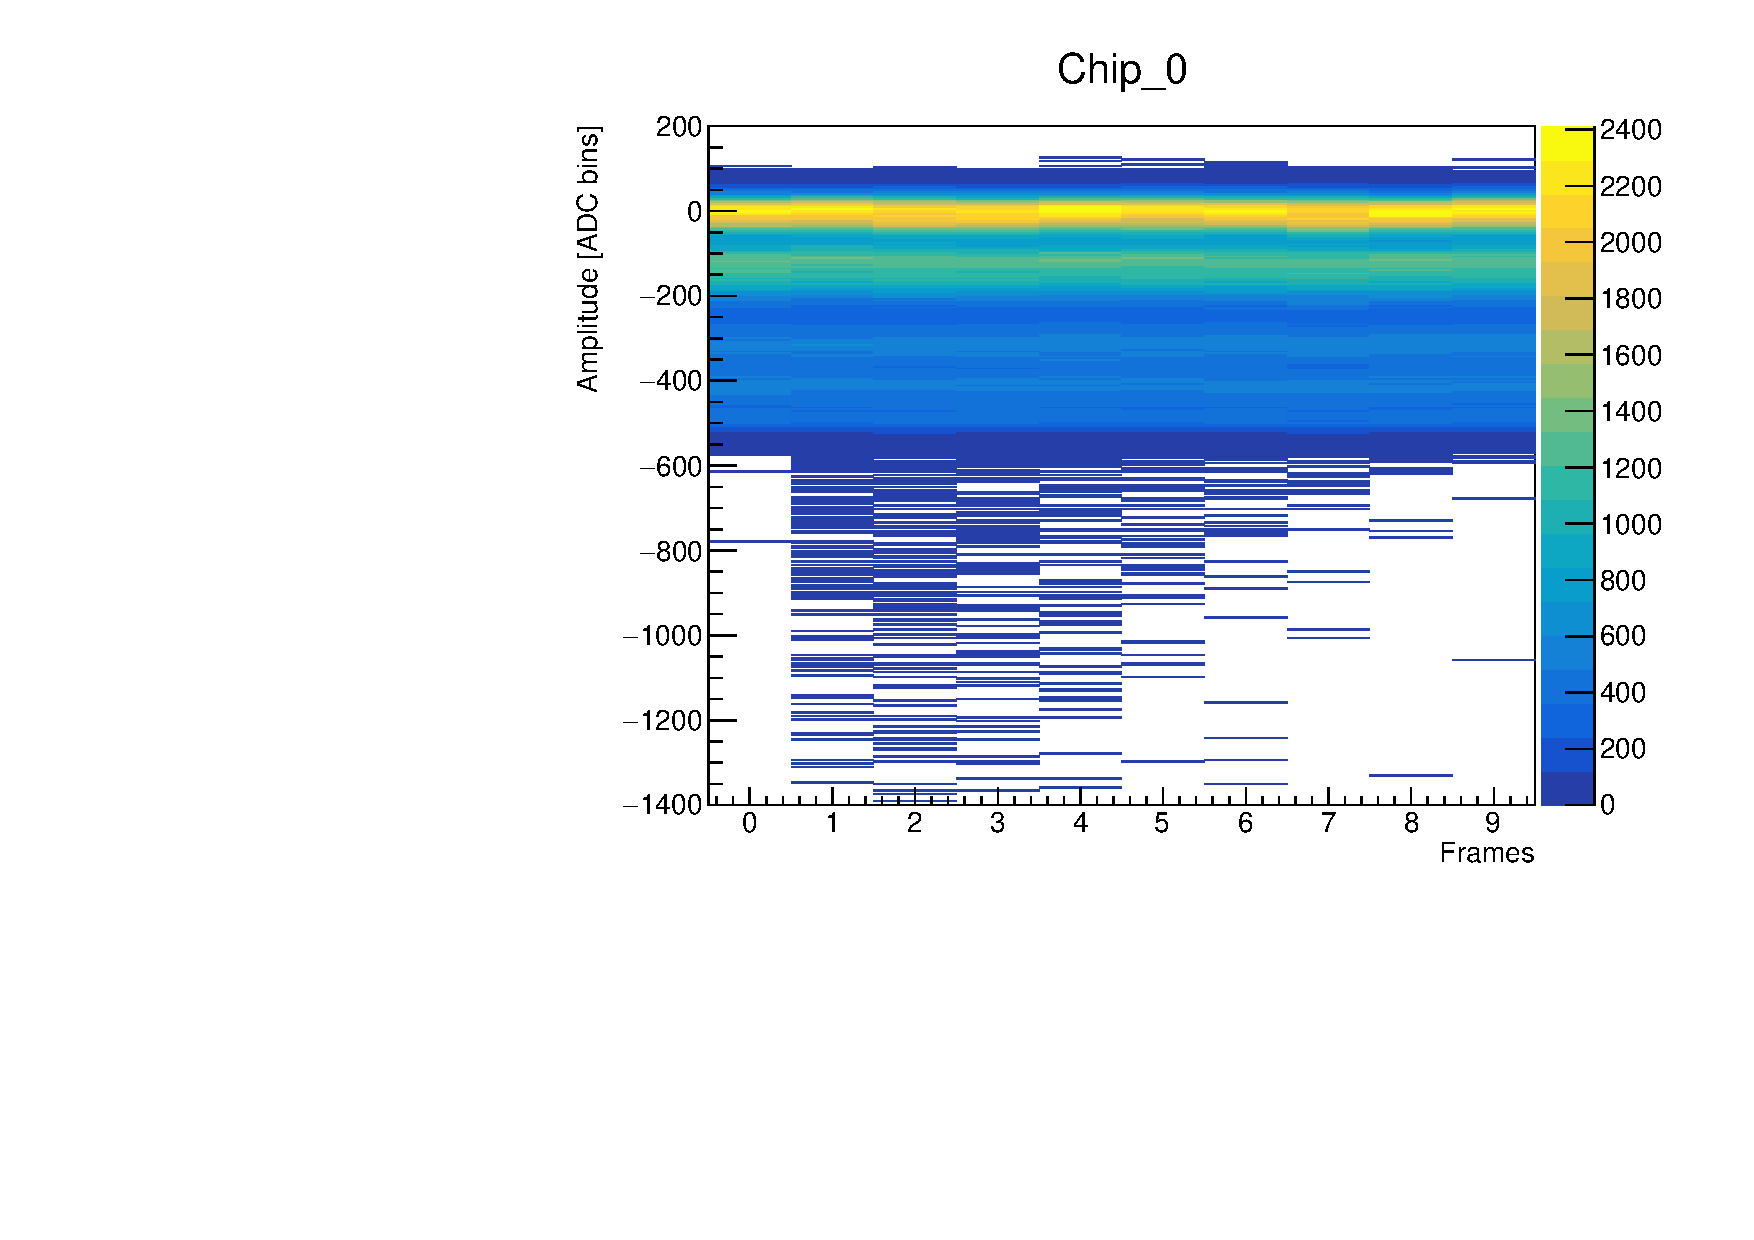
\includegraphics[width=\textwidth]{Chip_0_A2fr_hist}
\end{subfigure}
\begin{subfigure}[b]{0.45\textwidth}
	\centering
	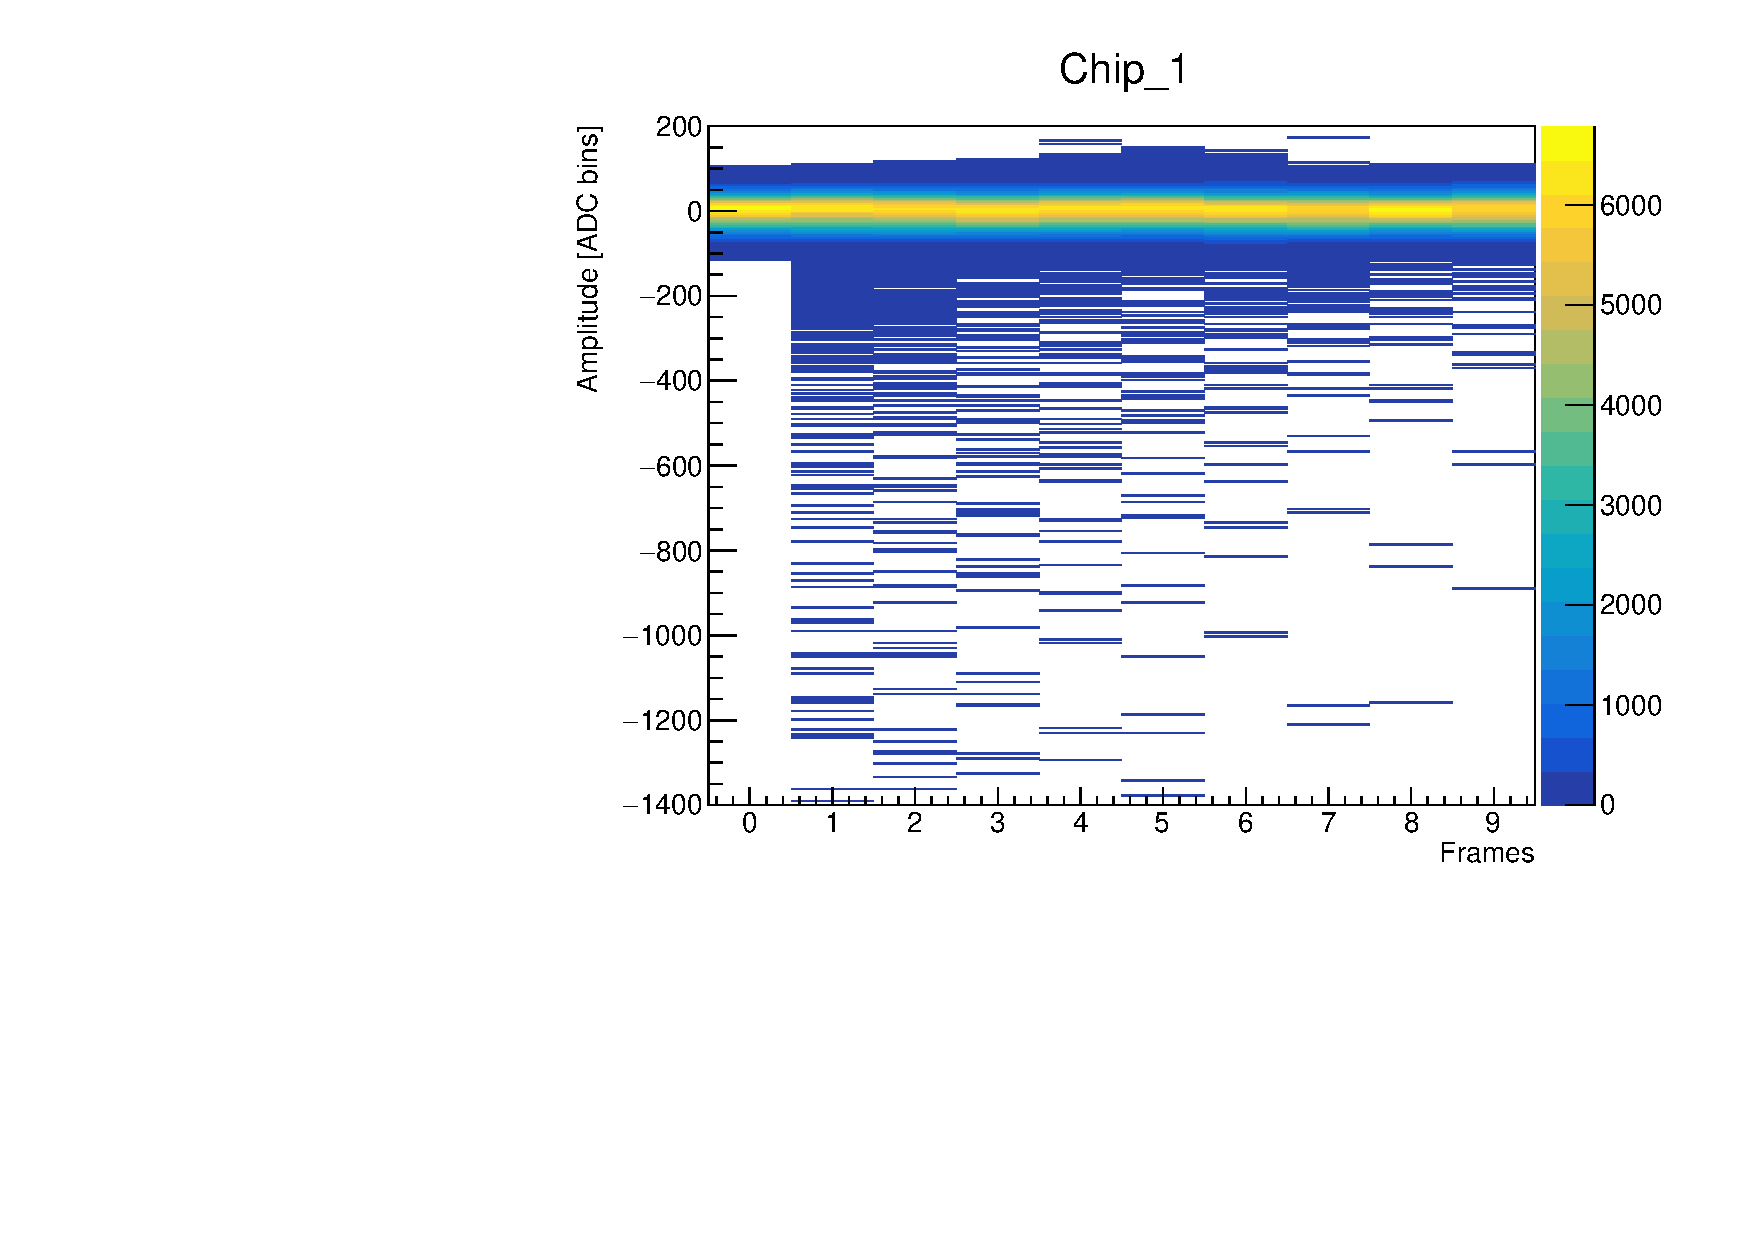
\includegraphics[width=\textwidth]{Chip_1_A2fr_hist}
\end{subfigure}
\begin{subfigure}[b]{0.45\textwidth}
	\centering
	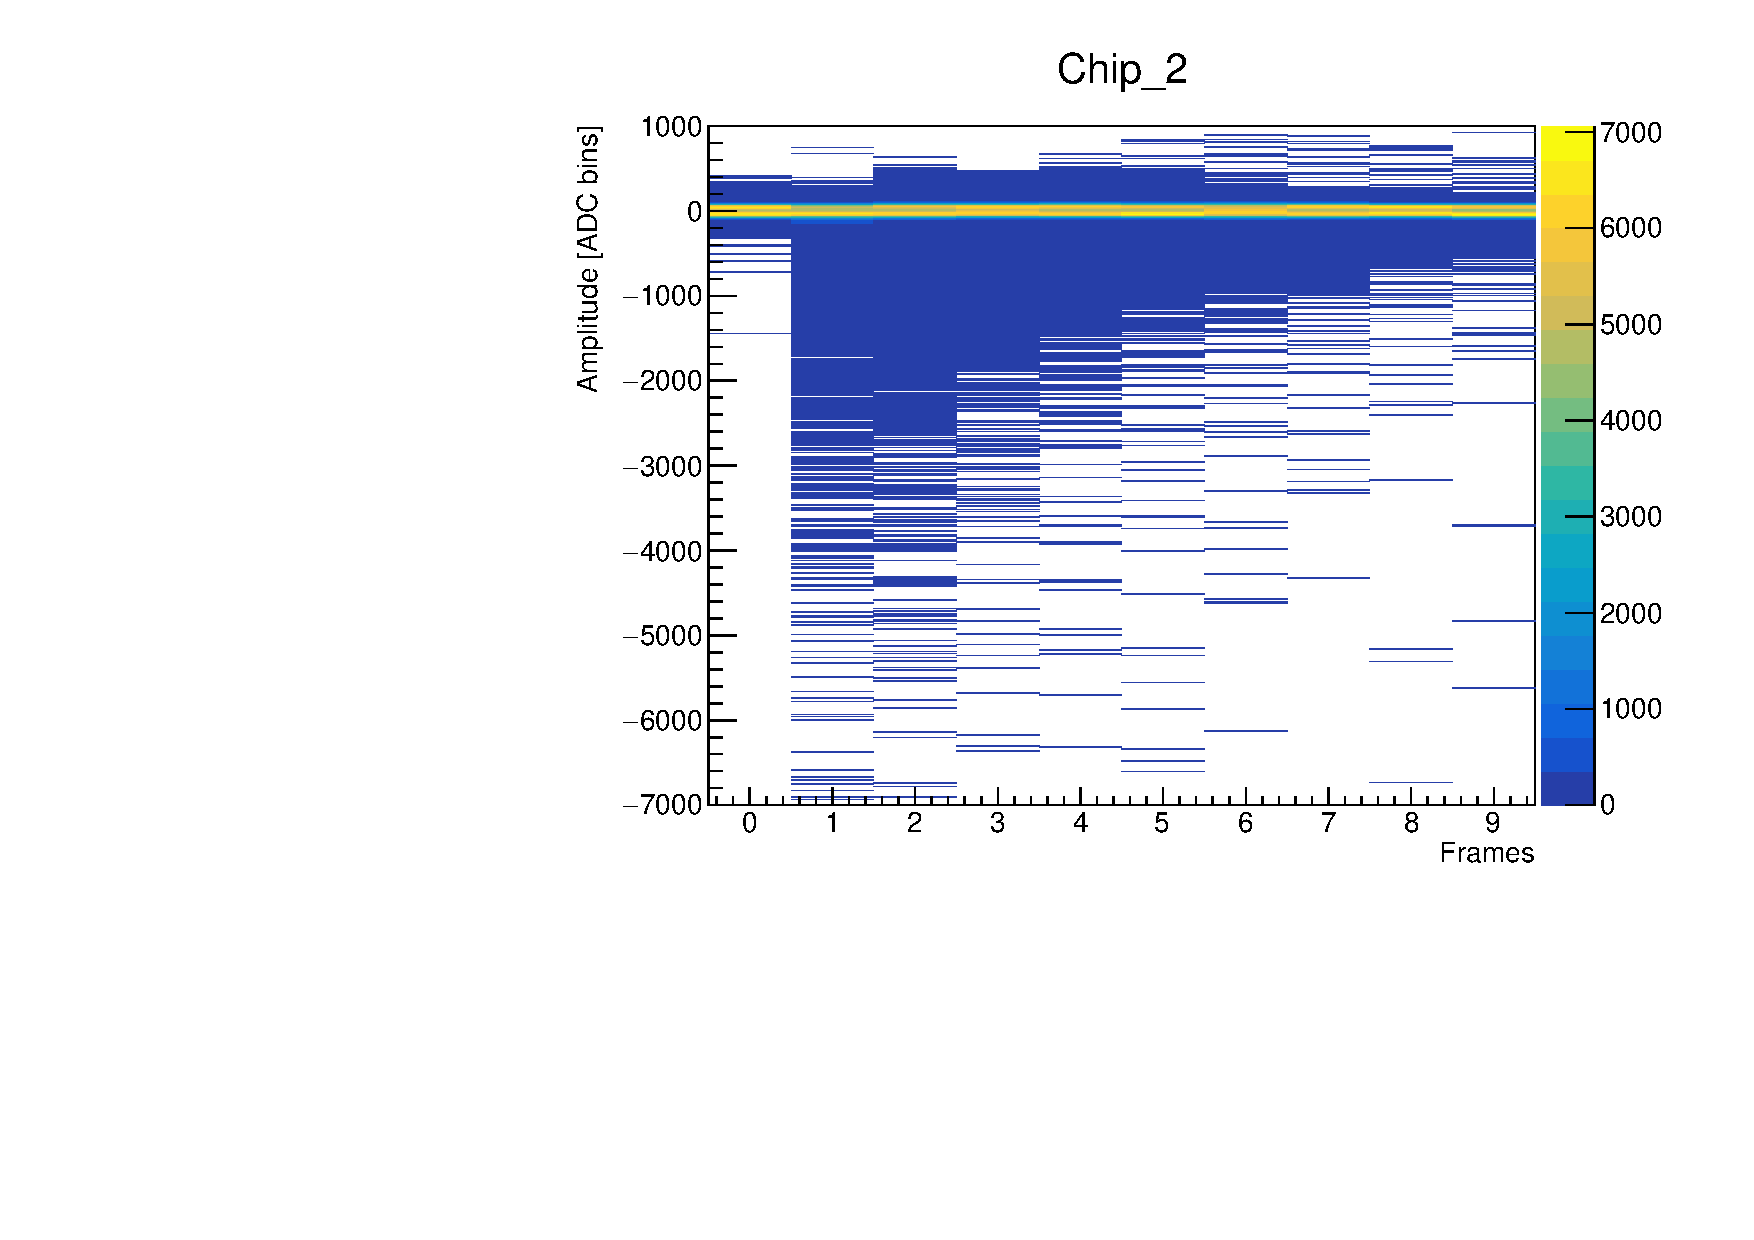
\includegraphics[width=\textwidth]{Chip_2_A2fr_hist}
\end{subfigure}
\begin{subfigure}[b]{0.45\textwidth}
	\centering
	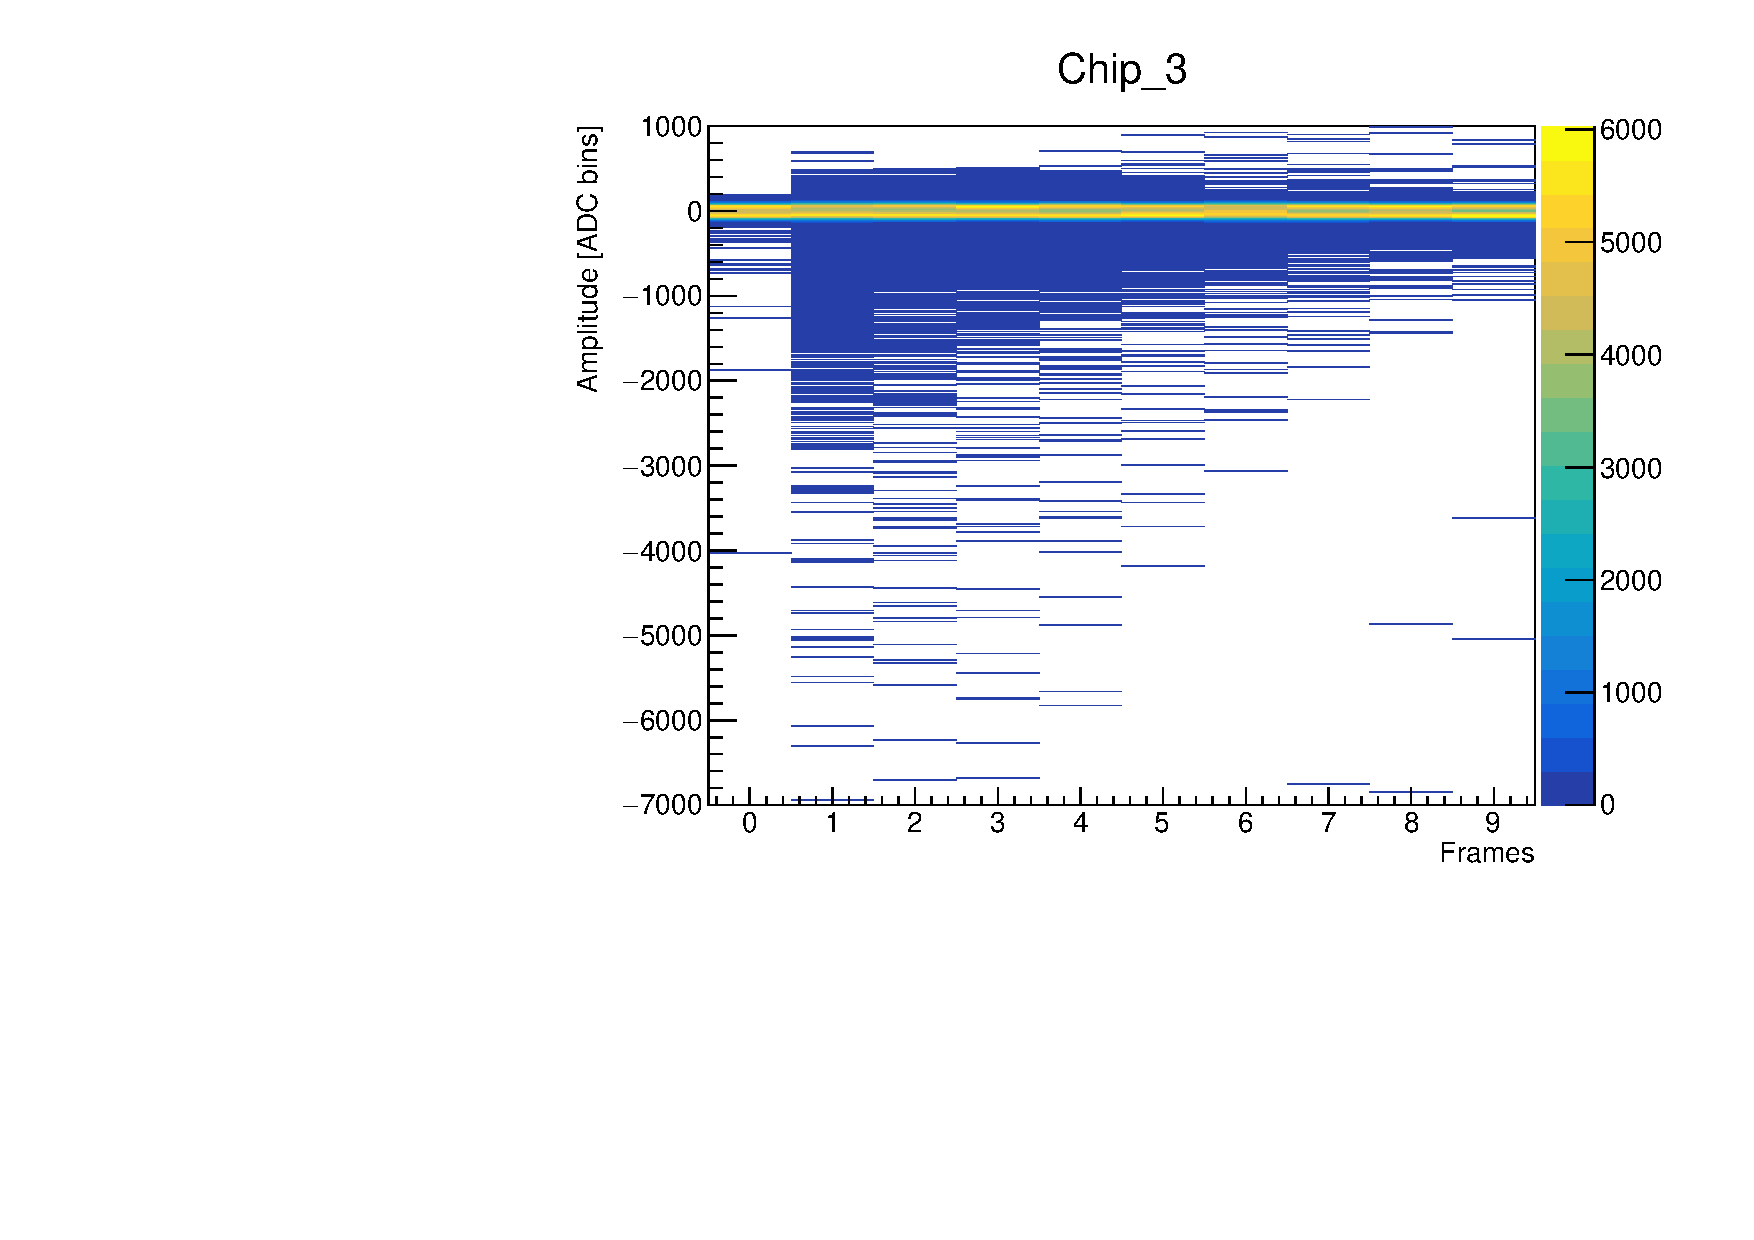
\includegraphics[width=\textwidth]{Chip_3_A2fr_hist}
\end{subfigure}

\begin{subfigure}[b]{0.45\textwidth}
	\centering
	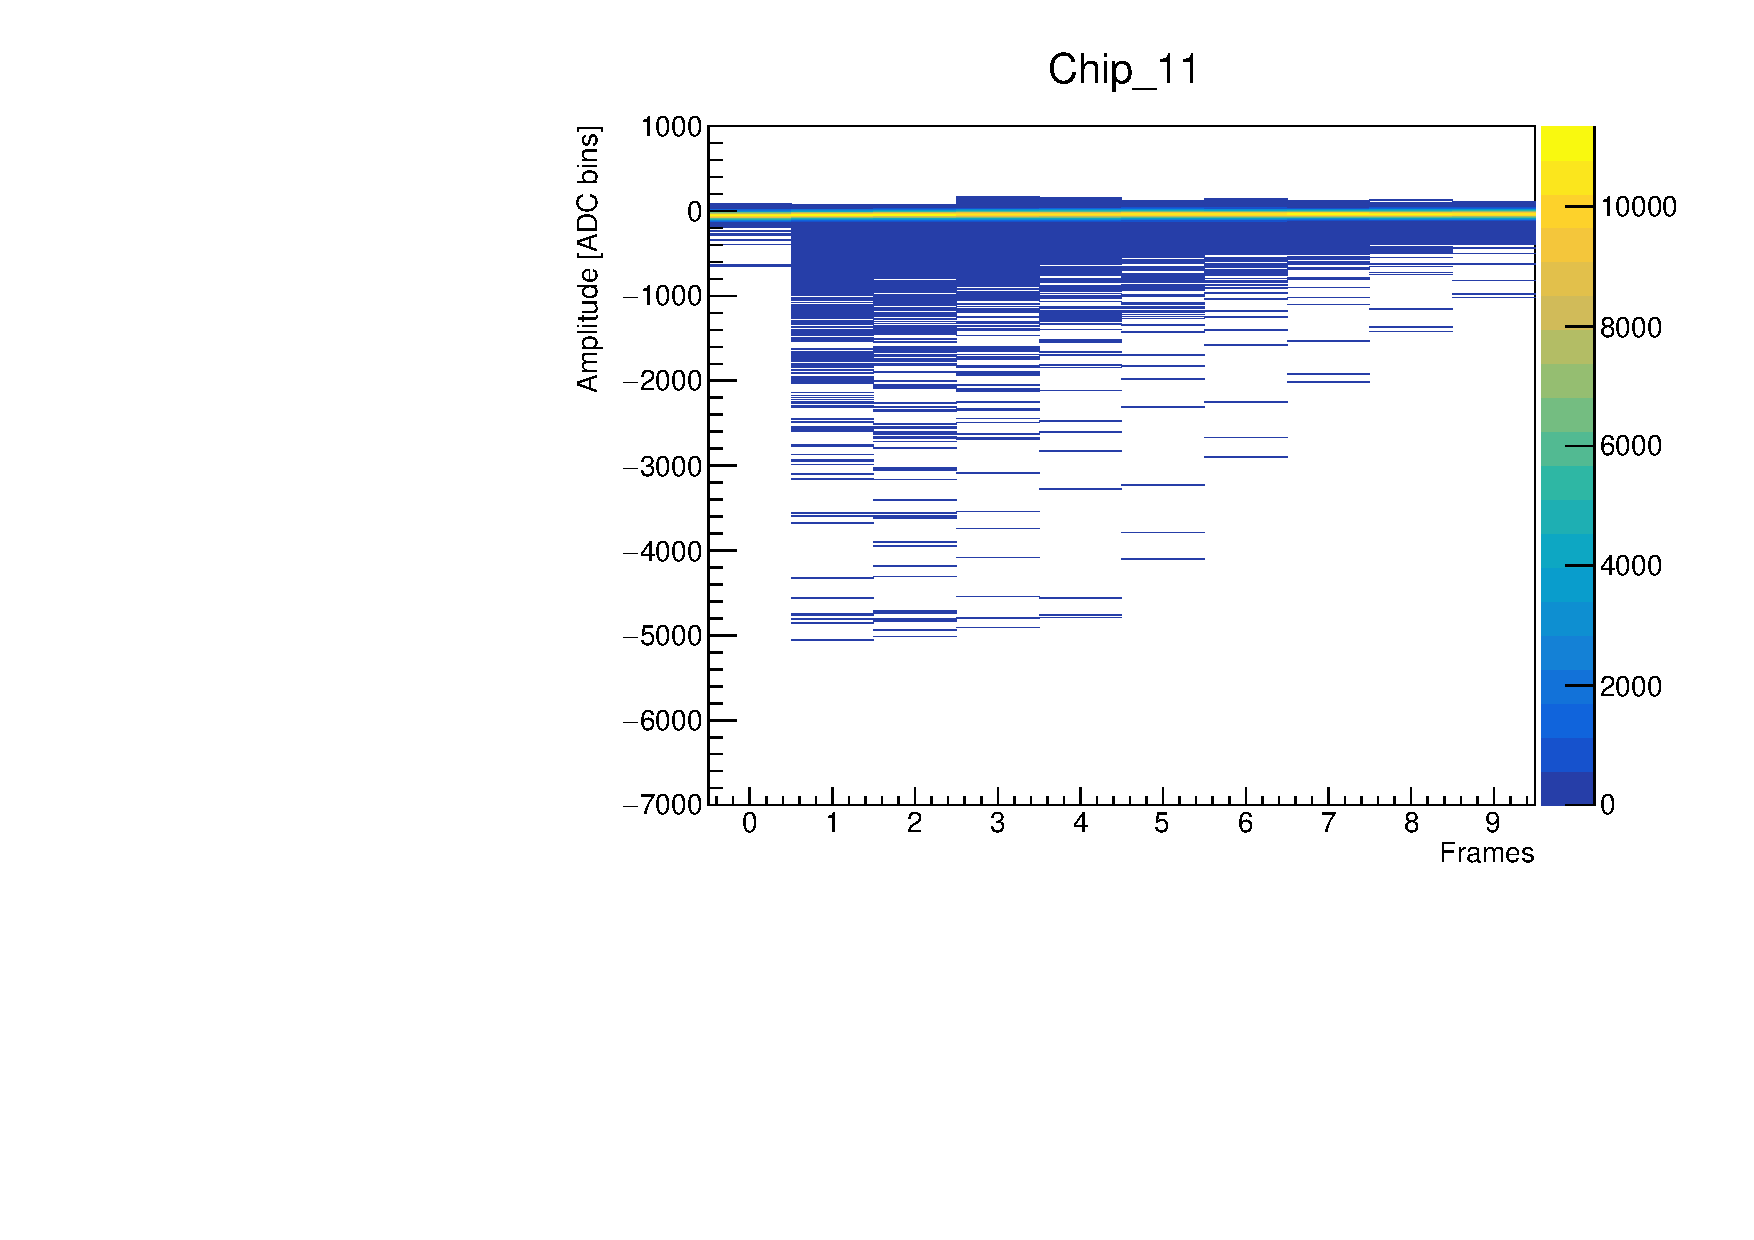
\includegraphics[width=\textwidth]{Chip_11_A2fr_hist}
\end{subfigure}
\begin{subfigure}[b]{0.45\textwidth}
	\centering
	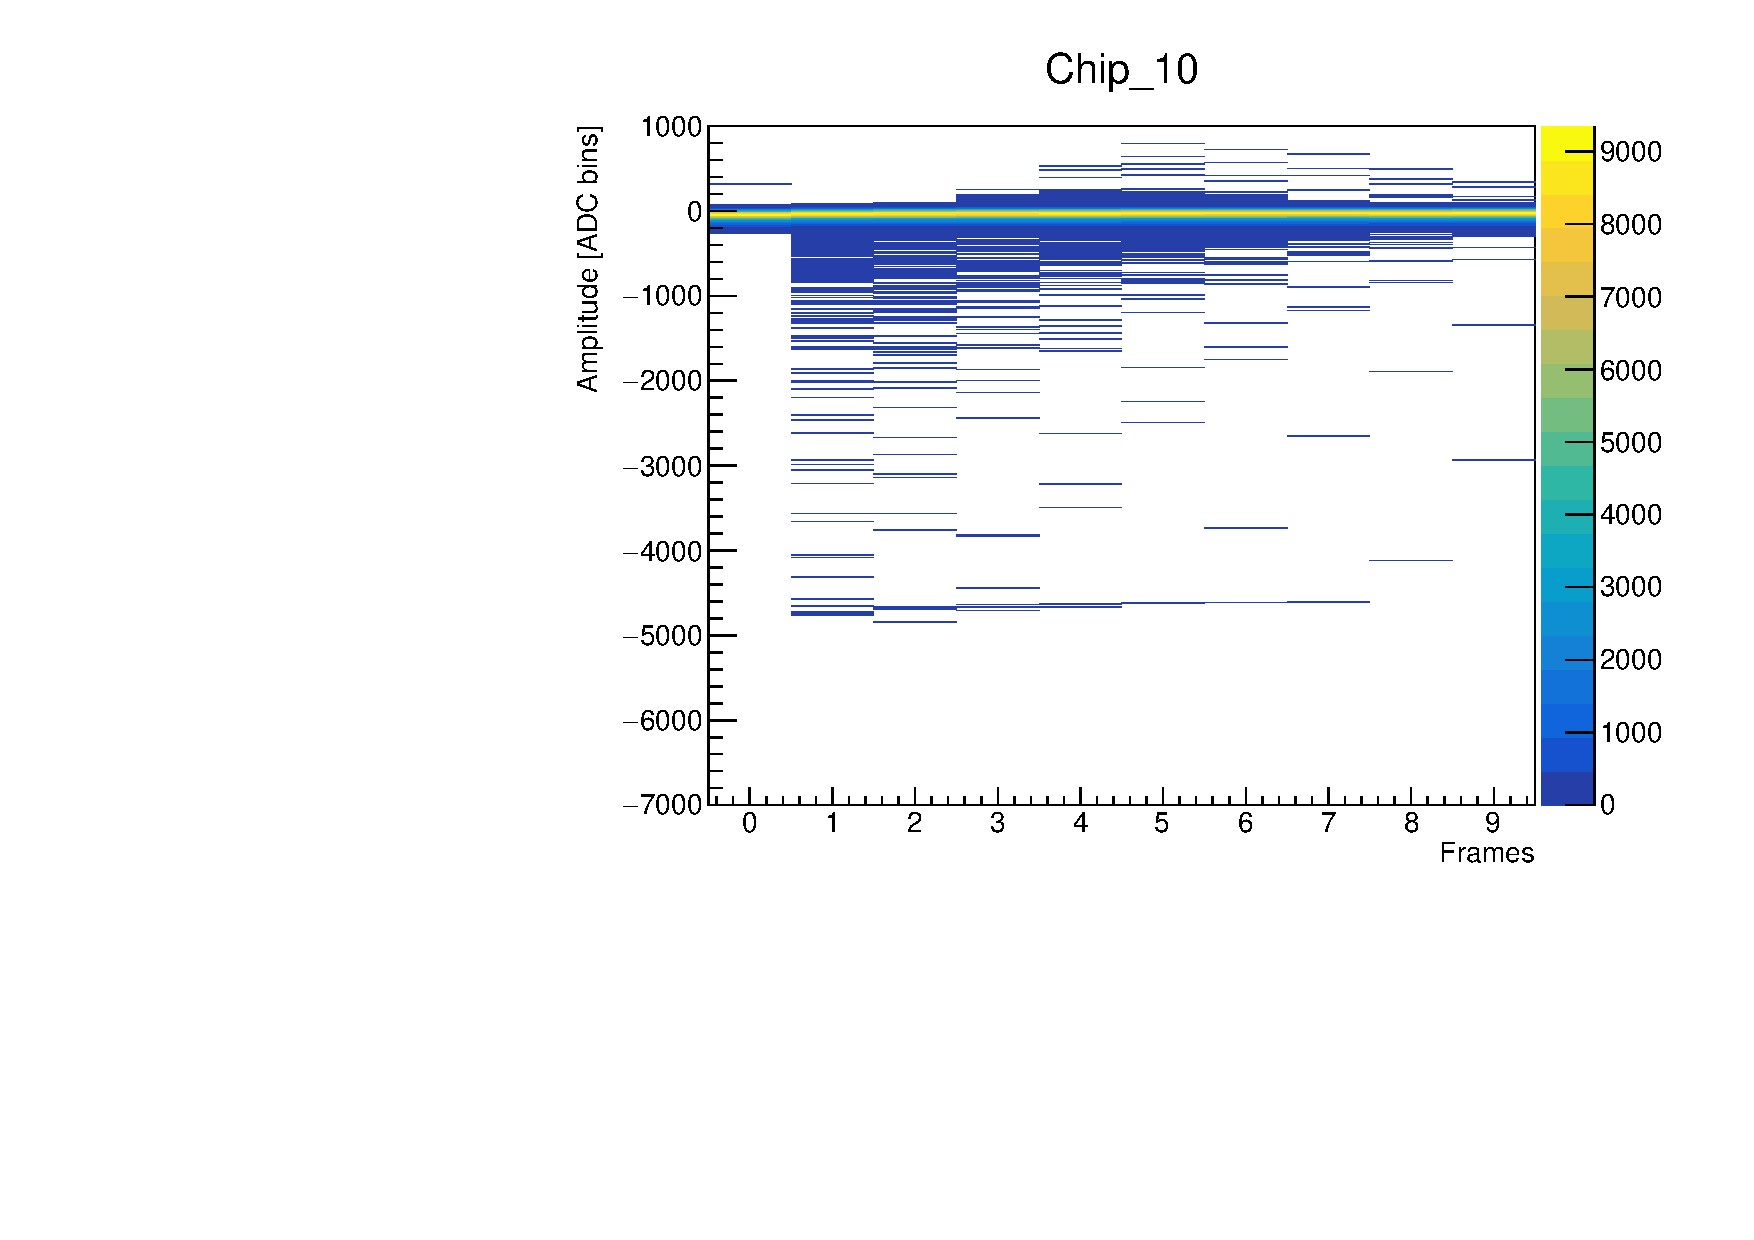
\includegraphics[width=\textwidth]{Chip_10_A2fr_hist}
\end{subfigure}
\begin{subfigure}[b]{0.45\textwidth}
	\centering
	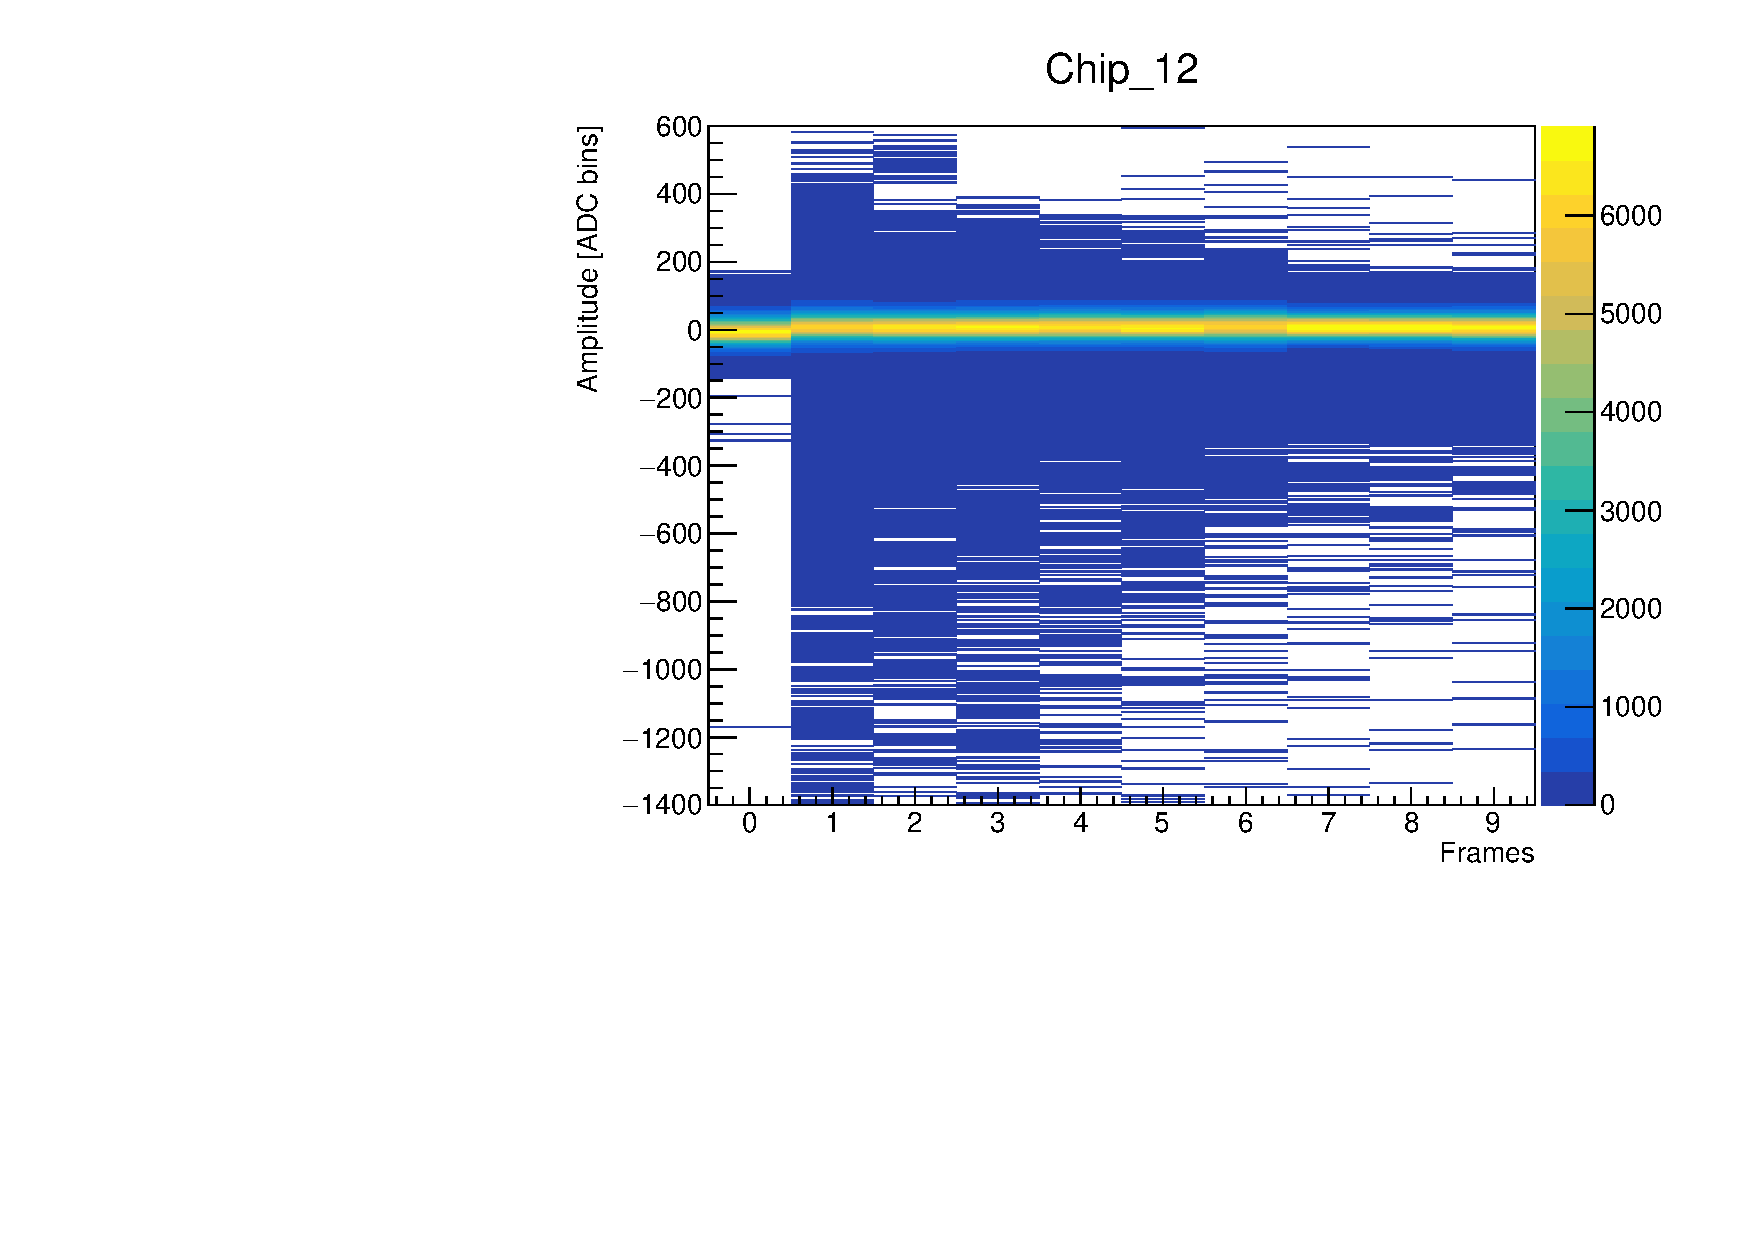
\includegraphics[width=\textwidth]{Chip_12_A2fr_hist}
\end{subfigure}
\caption{Совместные распределения событий по кадрам и амплитудам.}
\label{fig:h2d}
\end{figure}
\begin{figure}[h!]
	\centering
	\begin{subfigure}[t]{0.45\textwidth}
		\centering
		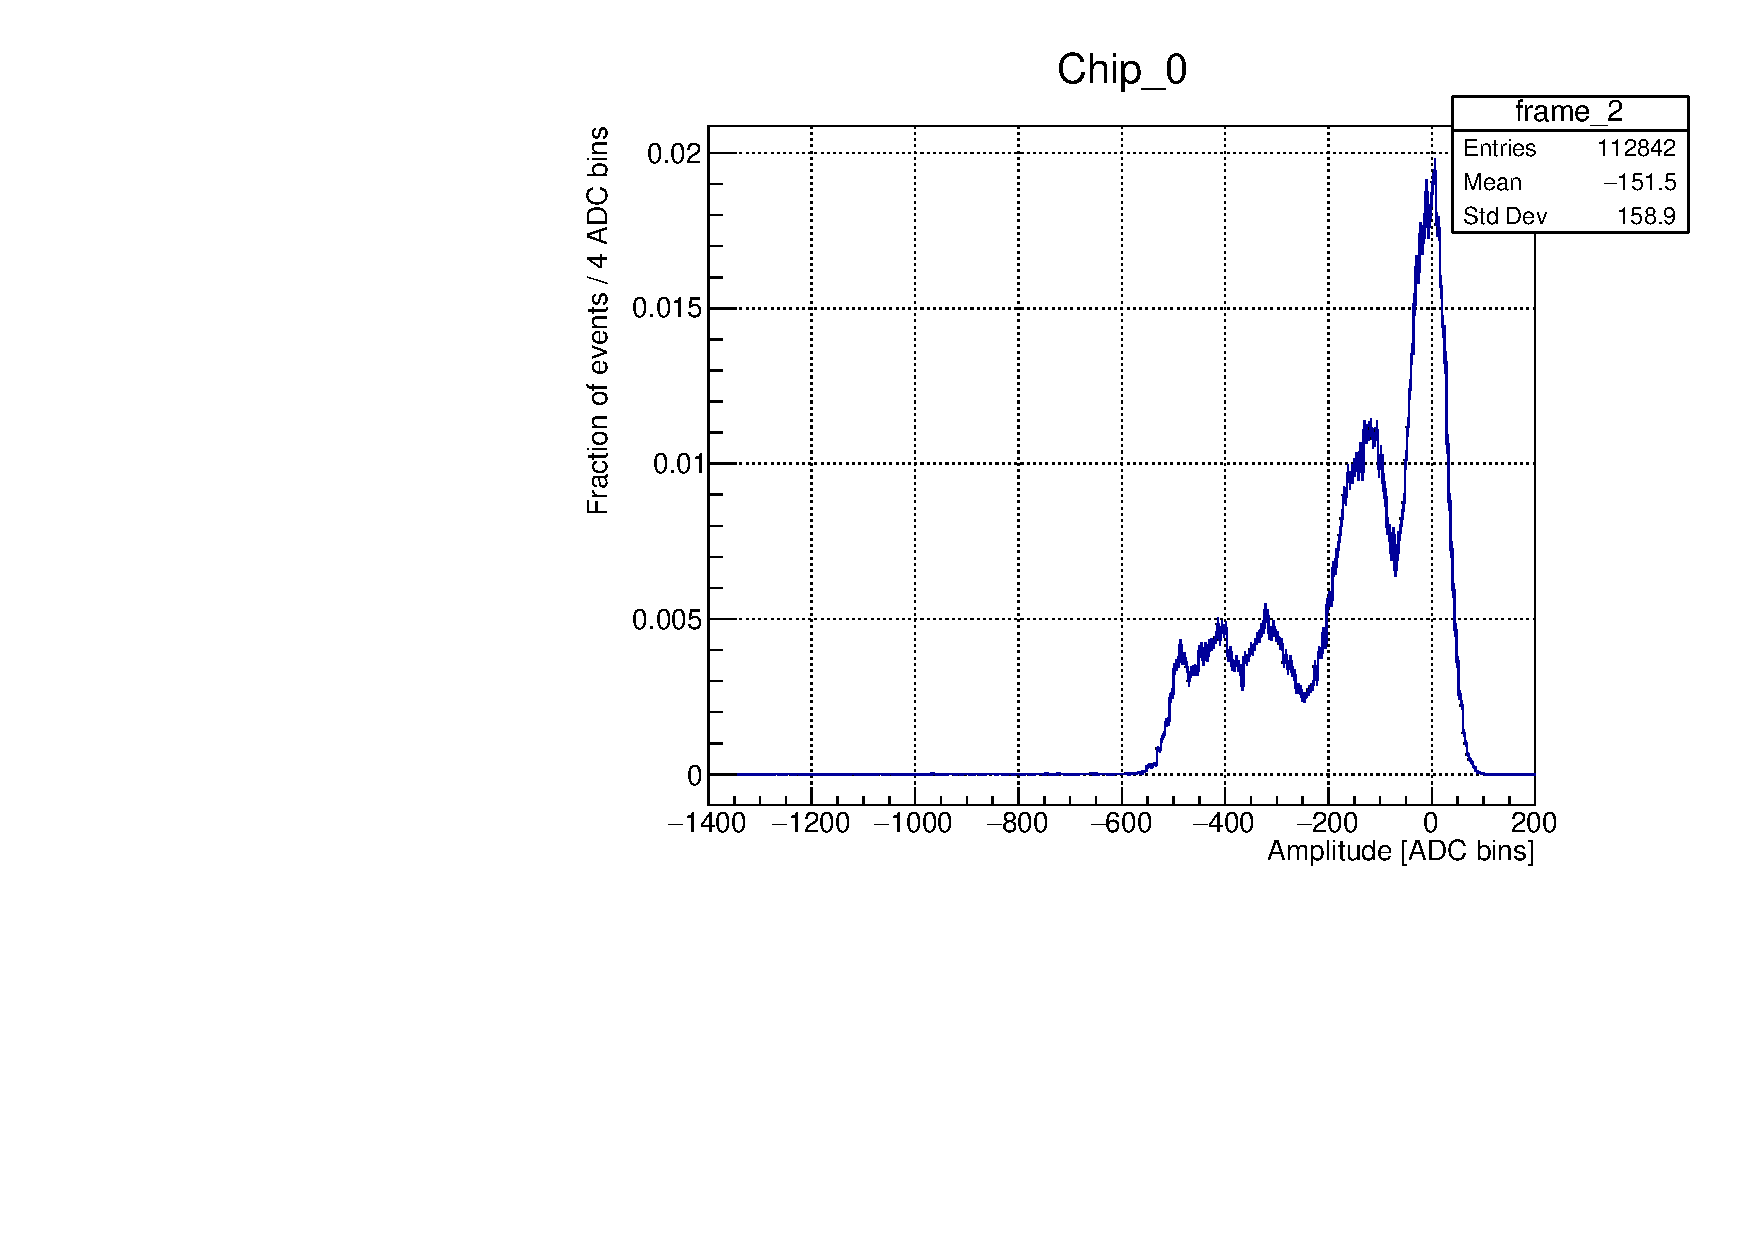
\includegraphics[width=\textwidth]{Chip_0_amp_hist}
	\end{subfigure}
	\begin{subfigure}[t]{0.45\textwidth}
		\centering
		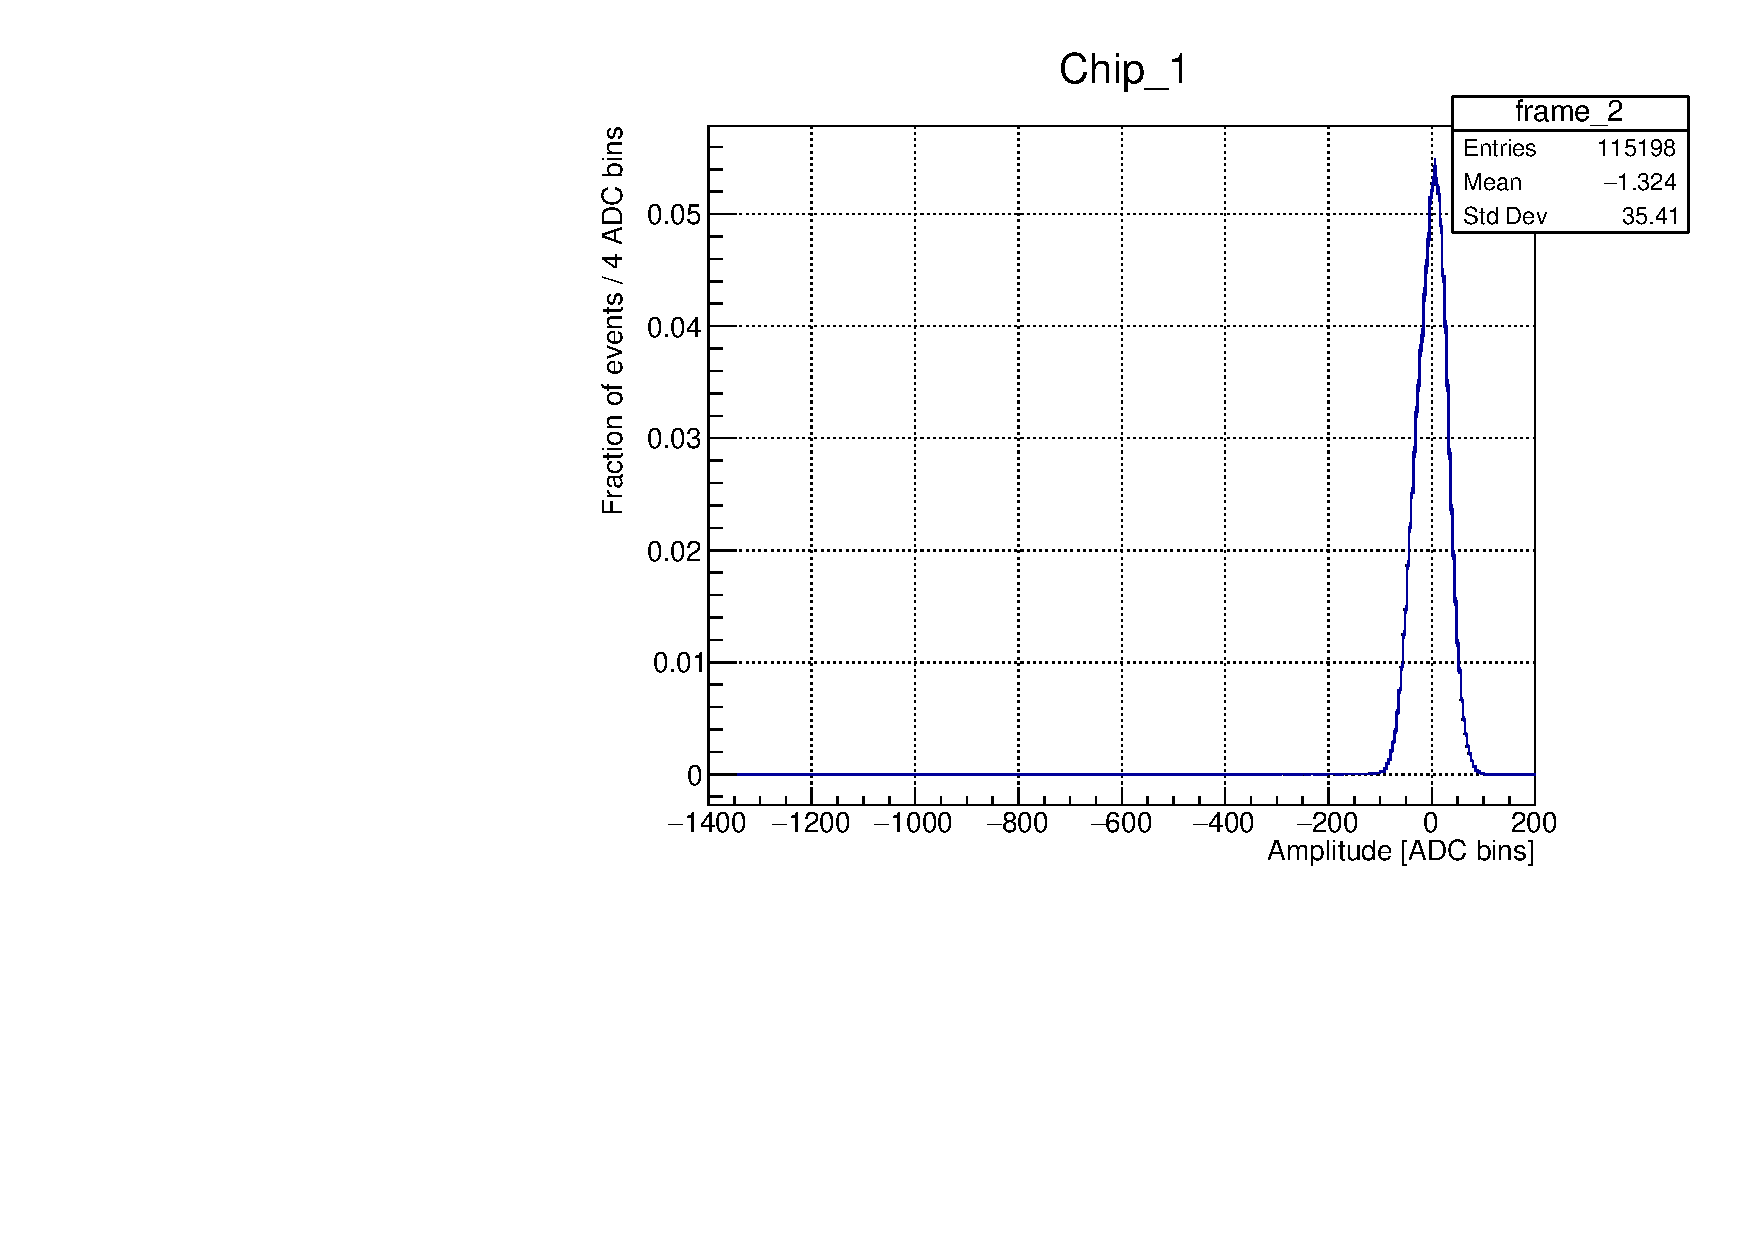
\includegraphics[width=\textwidth]{Chip_1_amp_hist}
	\end{subfigure}
	\begin{subfigure}[t]{0.45\textwidth}
		\centering
		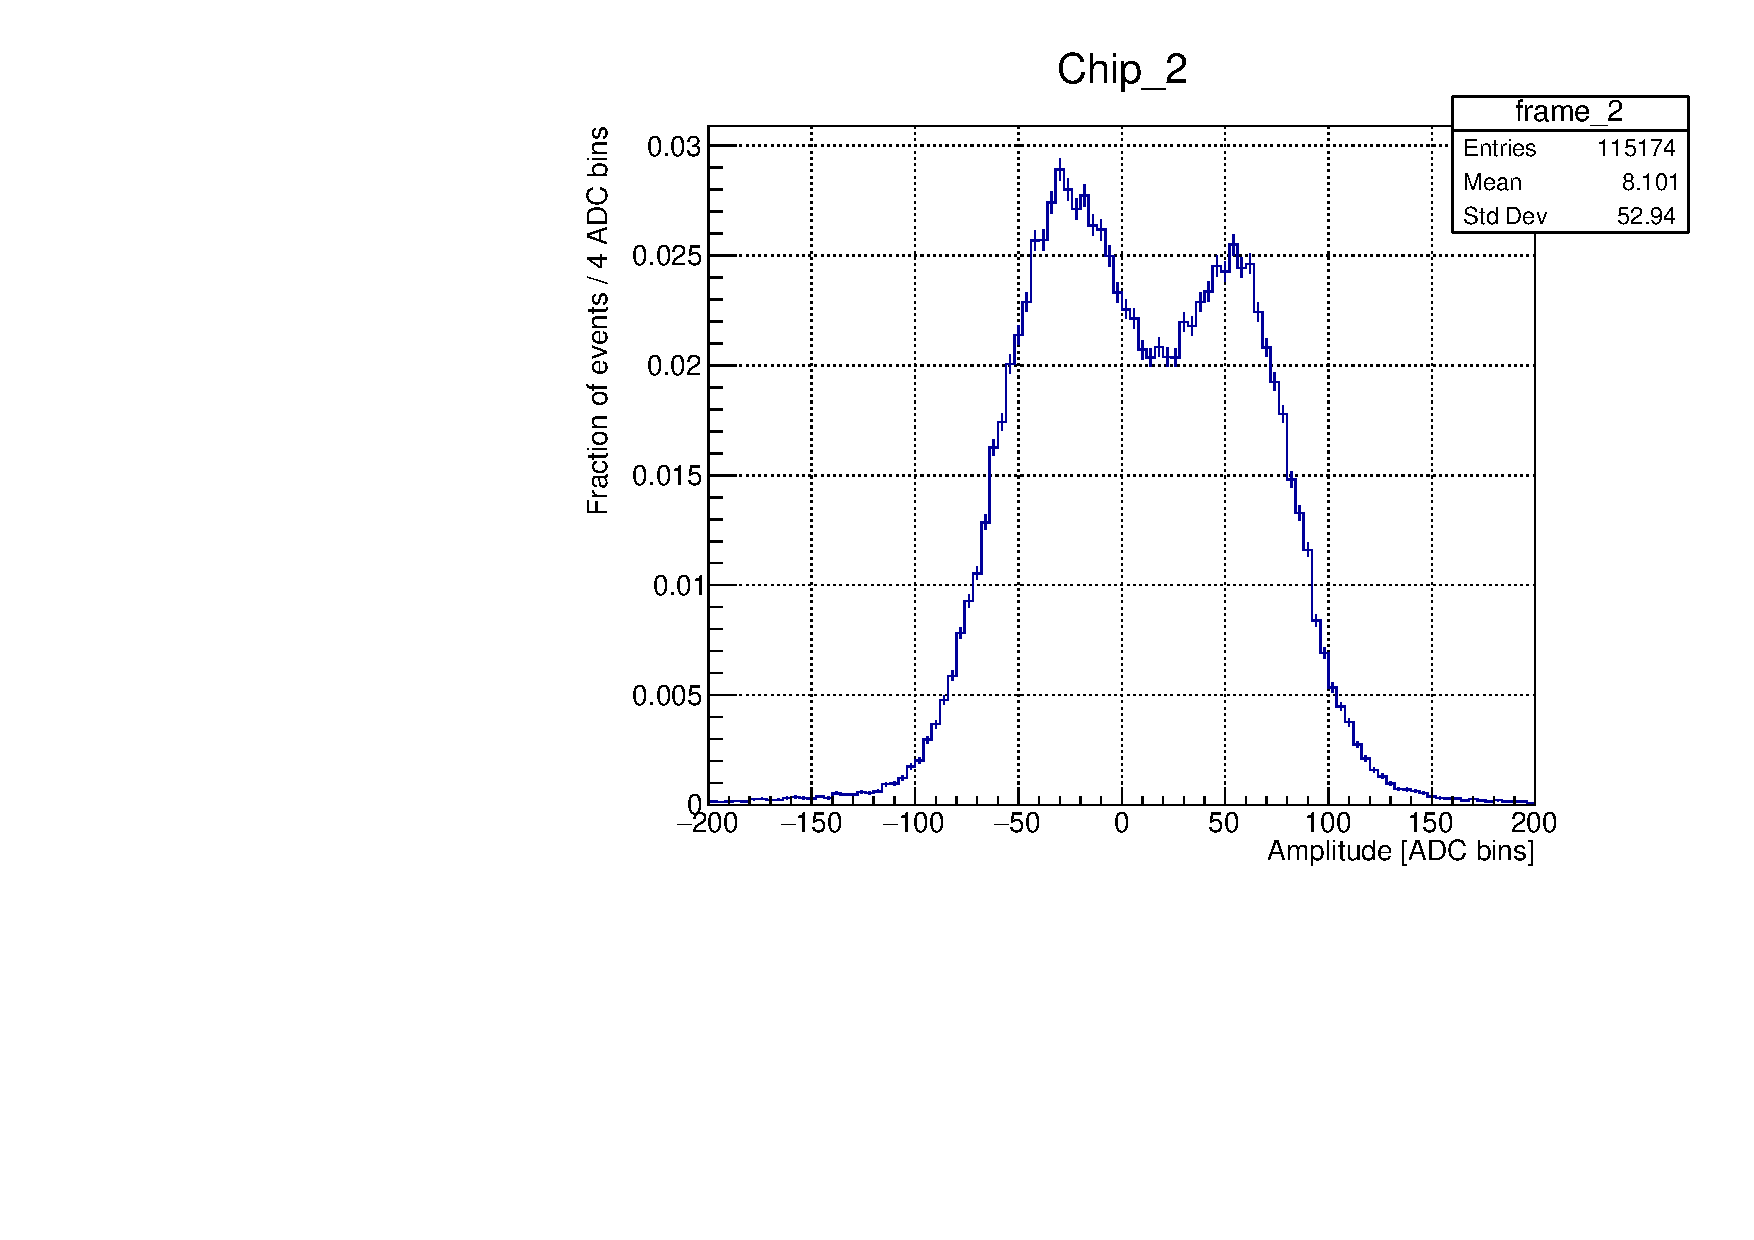
\includegraphics[width=\textwidth]{Chip_2_amp_hist}
	\end{subfigure}
	\begin{subfigure}[t]{0.45\textwidth}
		\centering
		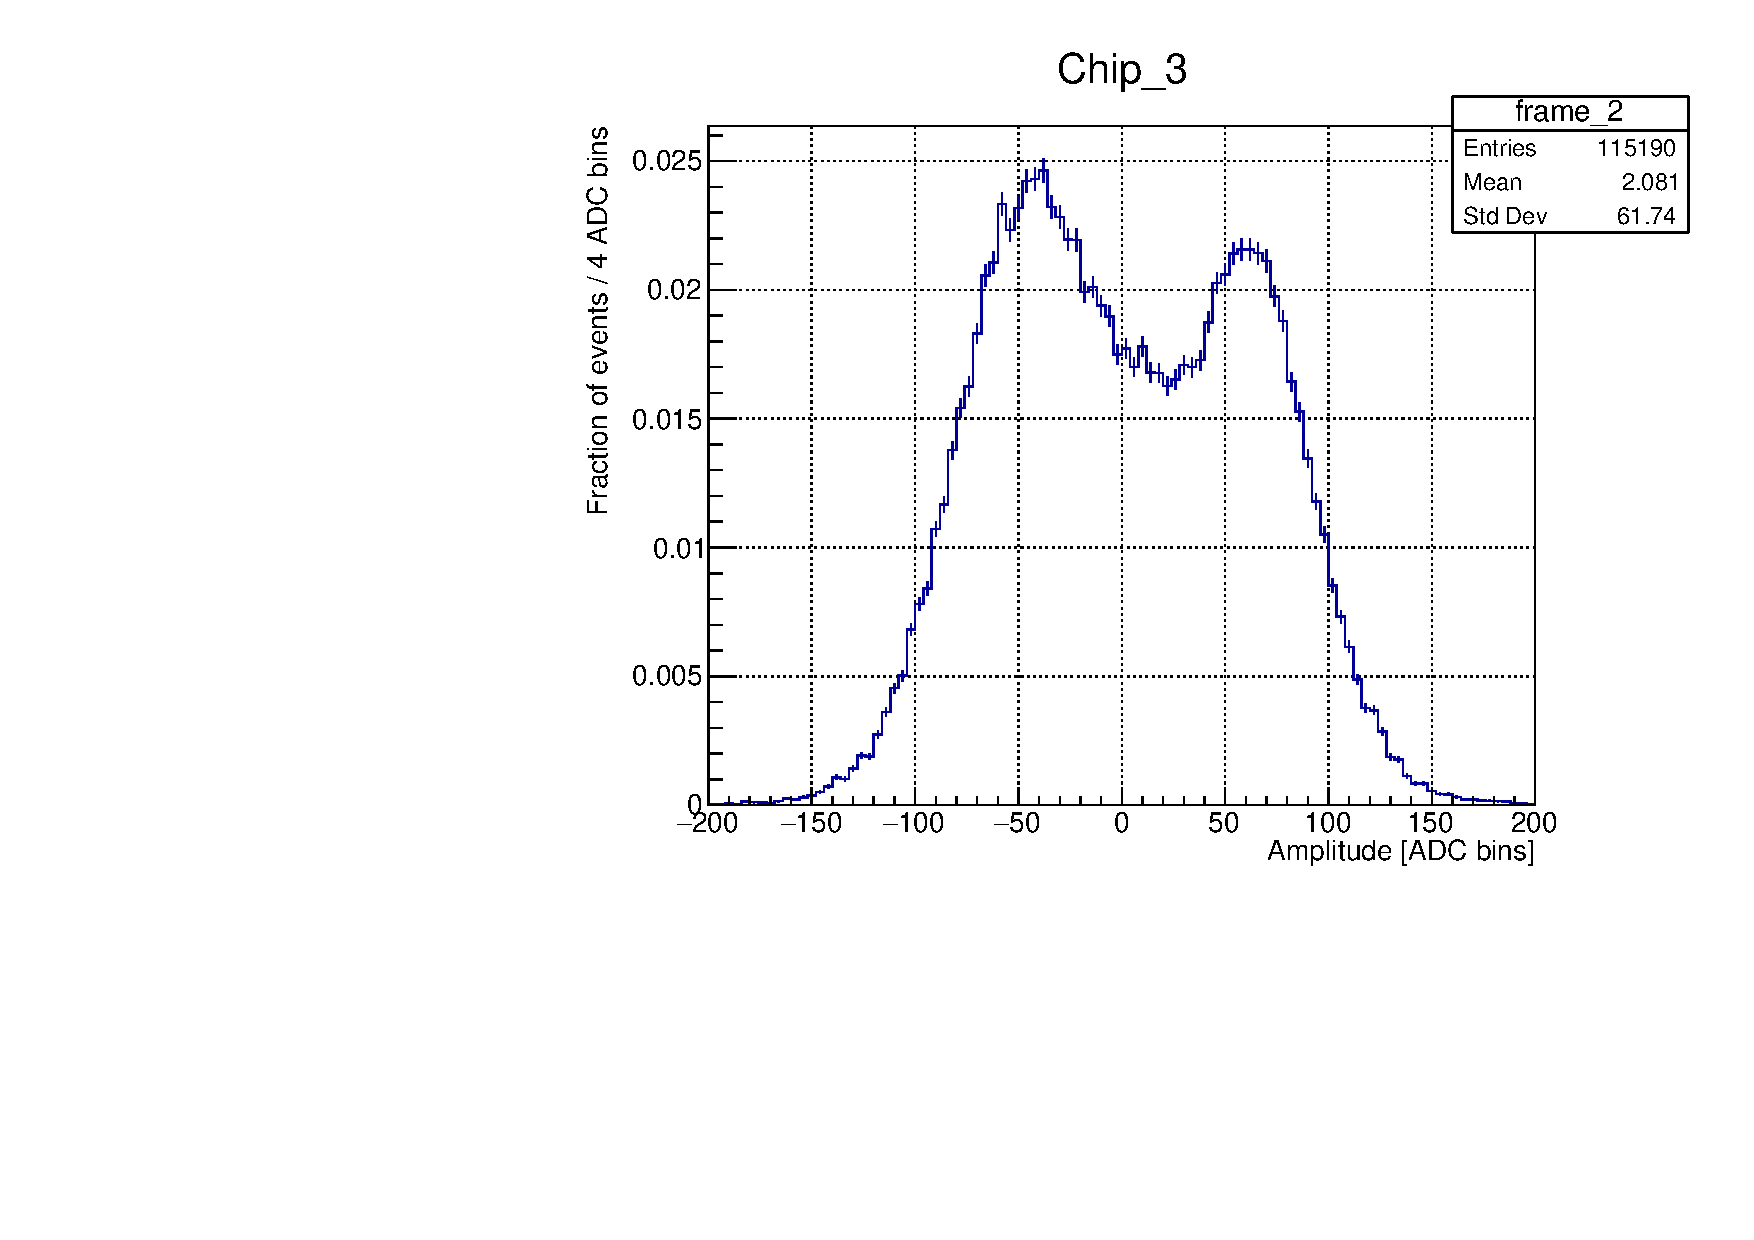
\includegraphics[width=\textwidth]{Chip_3_amp_hist}
	\end{subfigure}
	\begin{subfigure}[t]{0.45\textwidth}
		\centering
		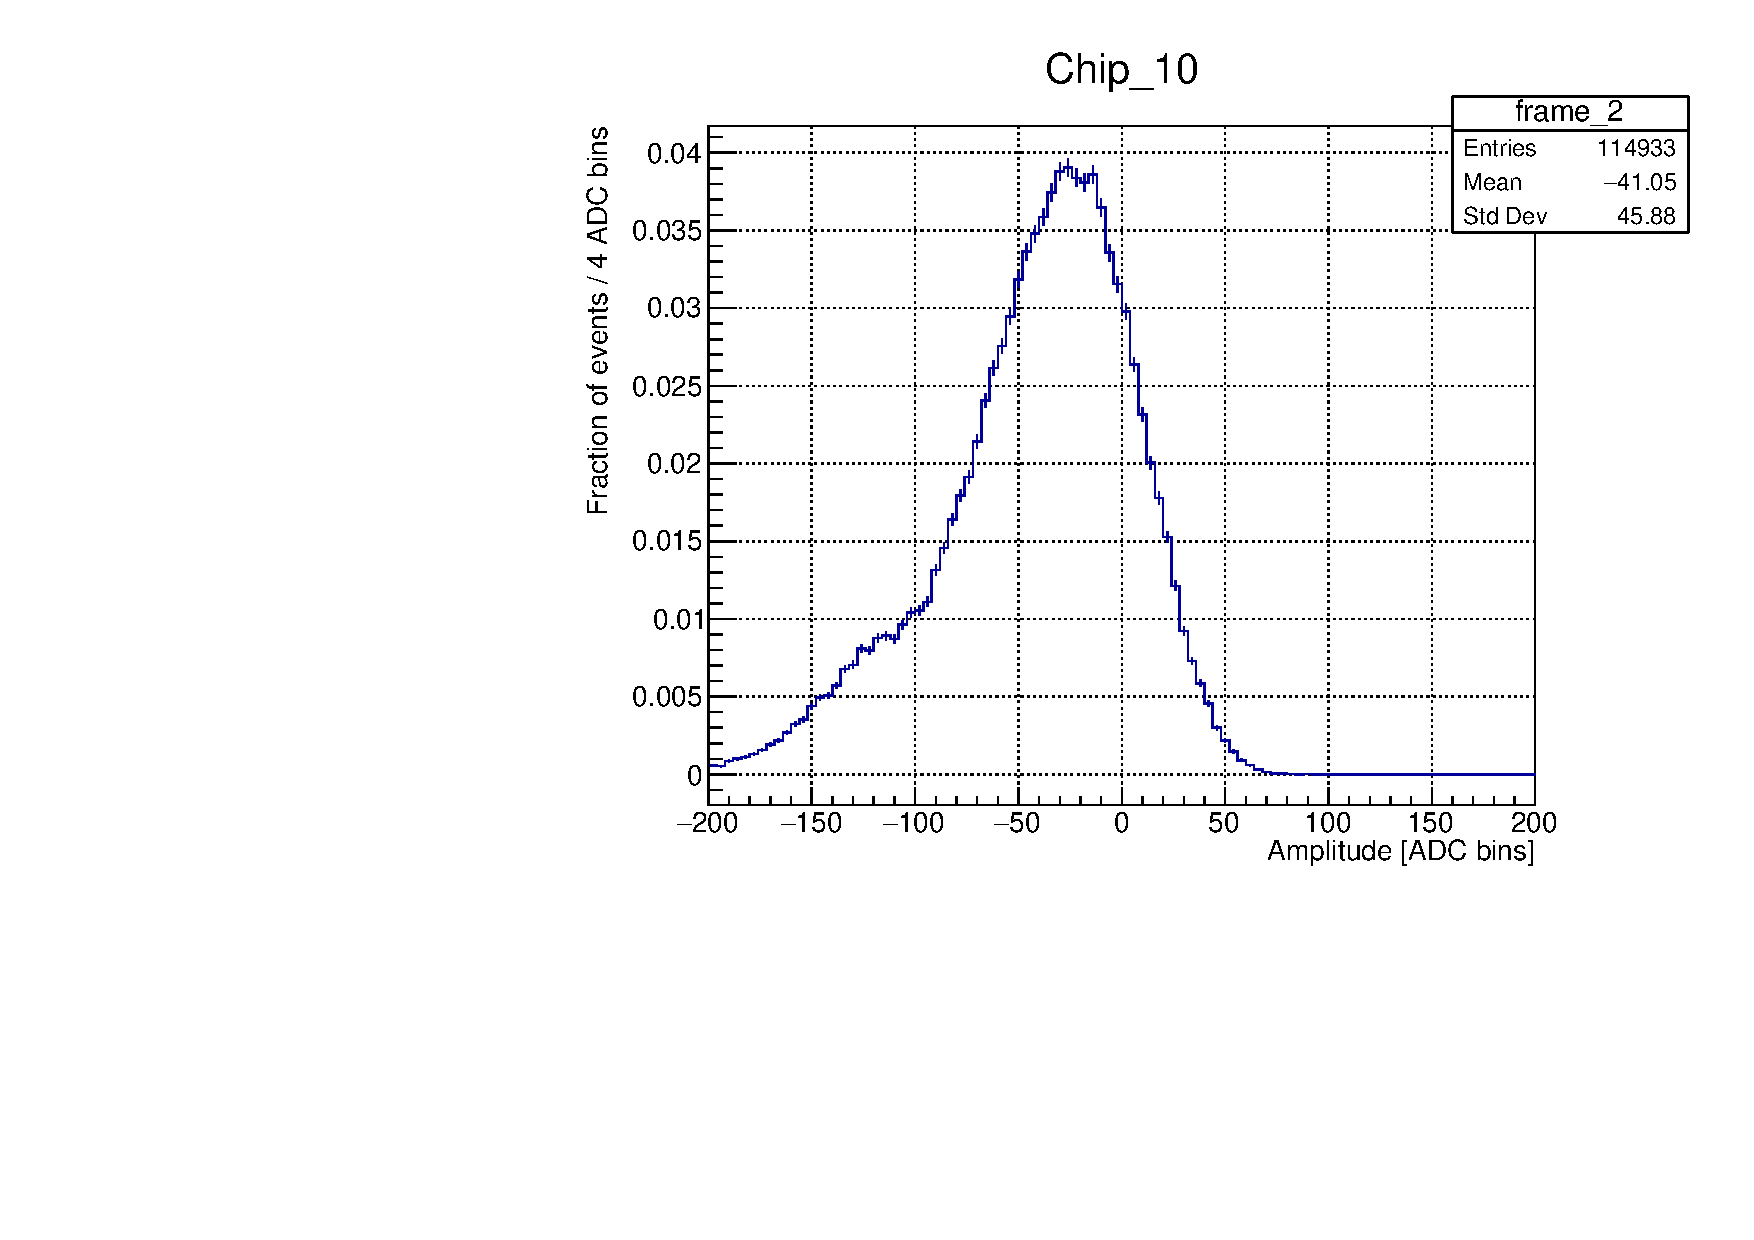
\includegraphics[width=\textwidth]{Chip_10_amp_hist}
	\end{subfigure}
	\begin{subfigure}[t]{0.45\textwidth}
		\centering
		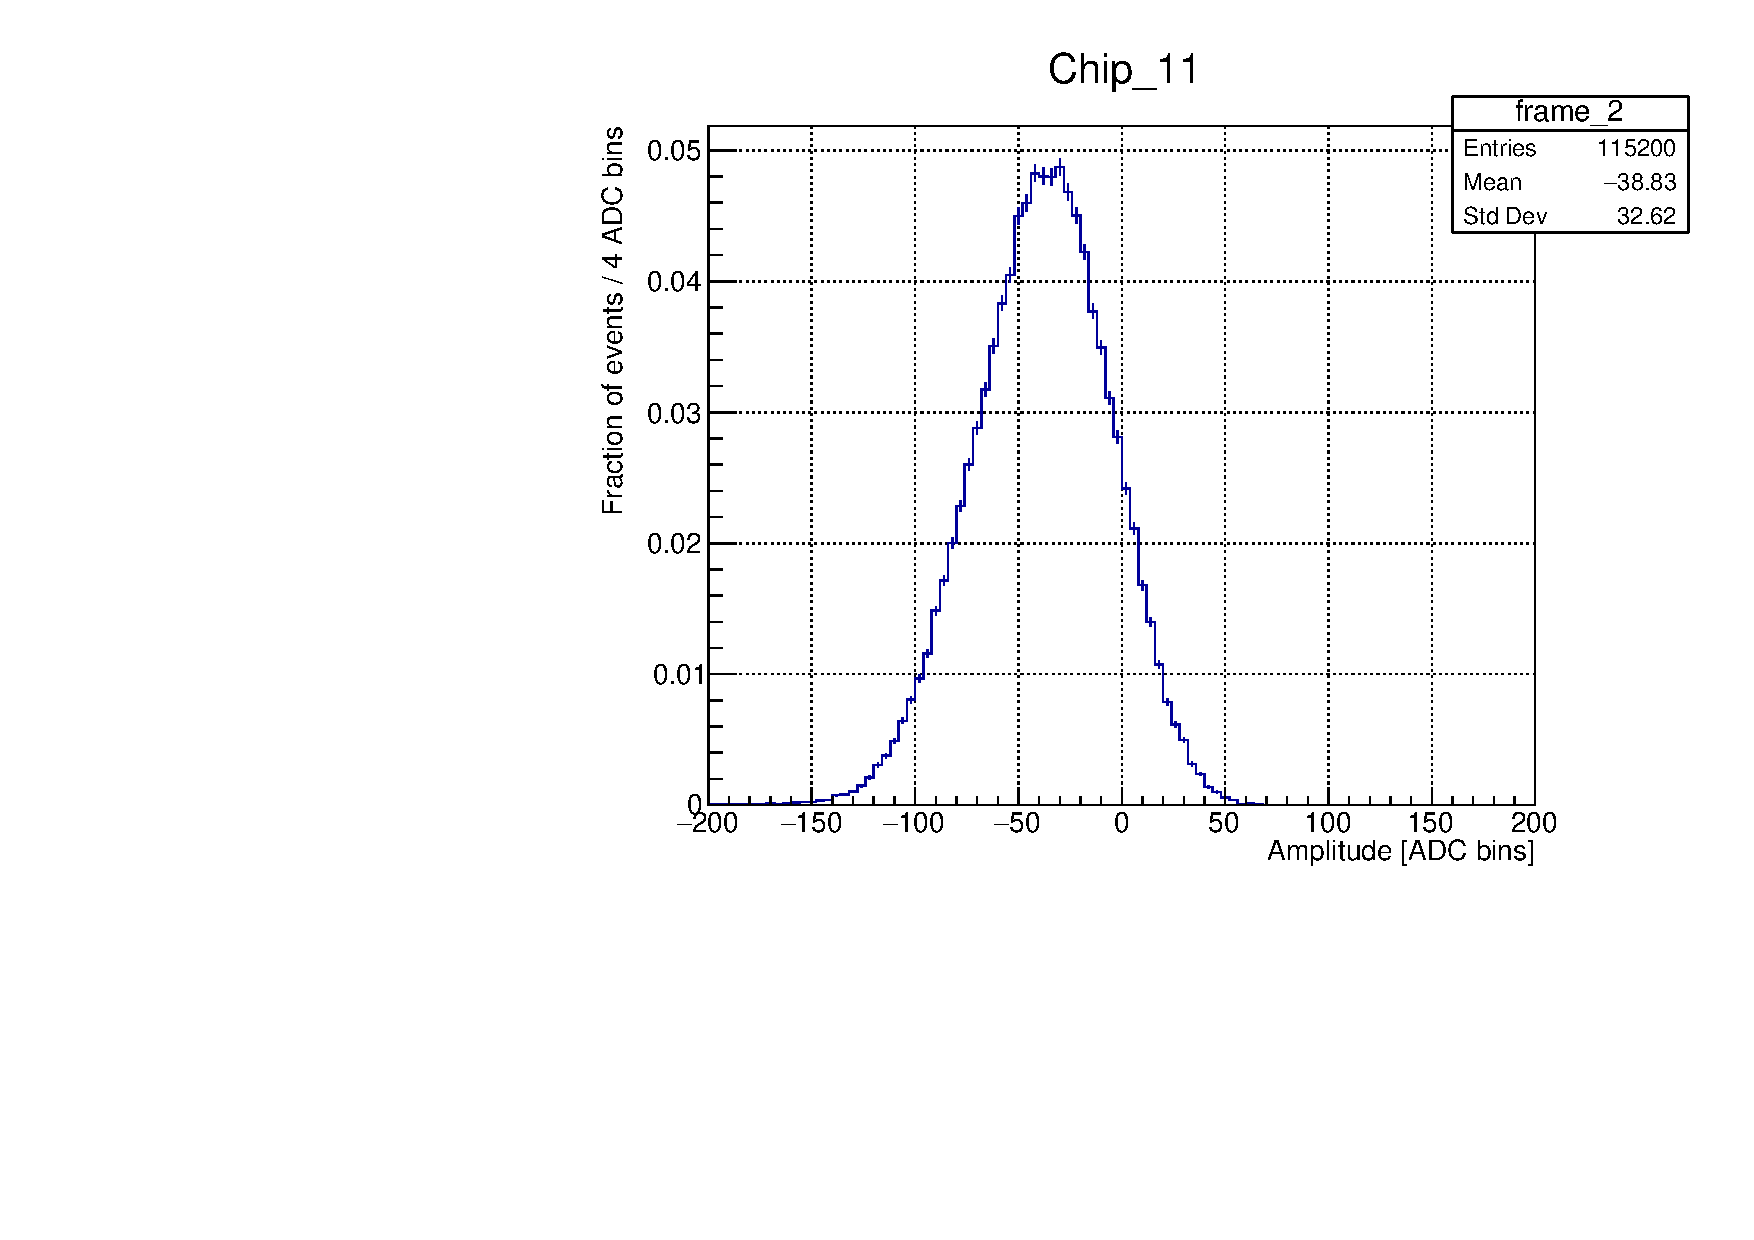
\includegraphics[width=\textwidth]{Chip_11_amp_hist}
	\end{subfigure}
	\begin{subfigure}[t]{0.45\textwidth}
		\centering
		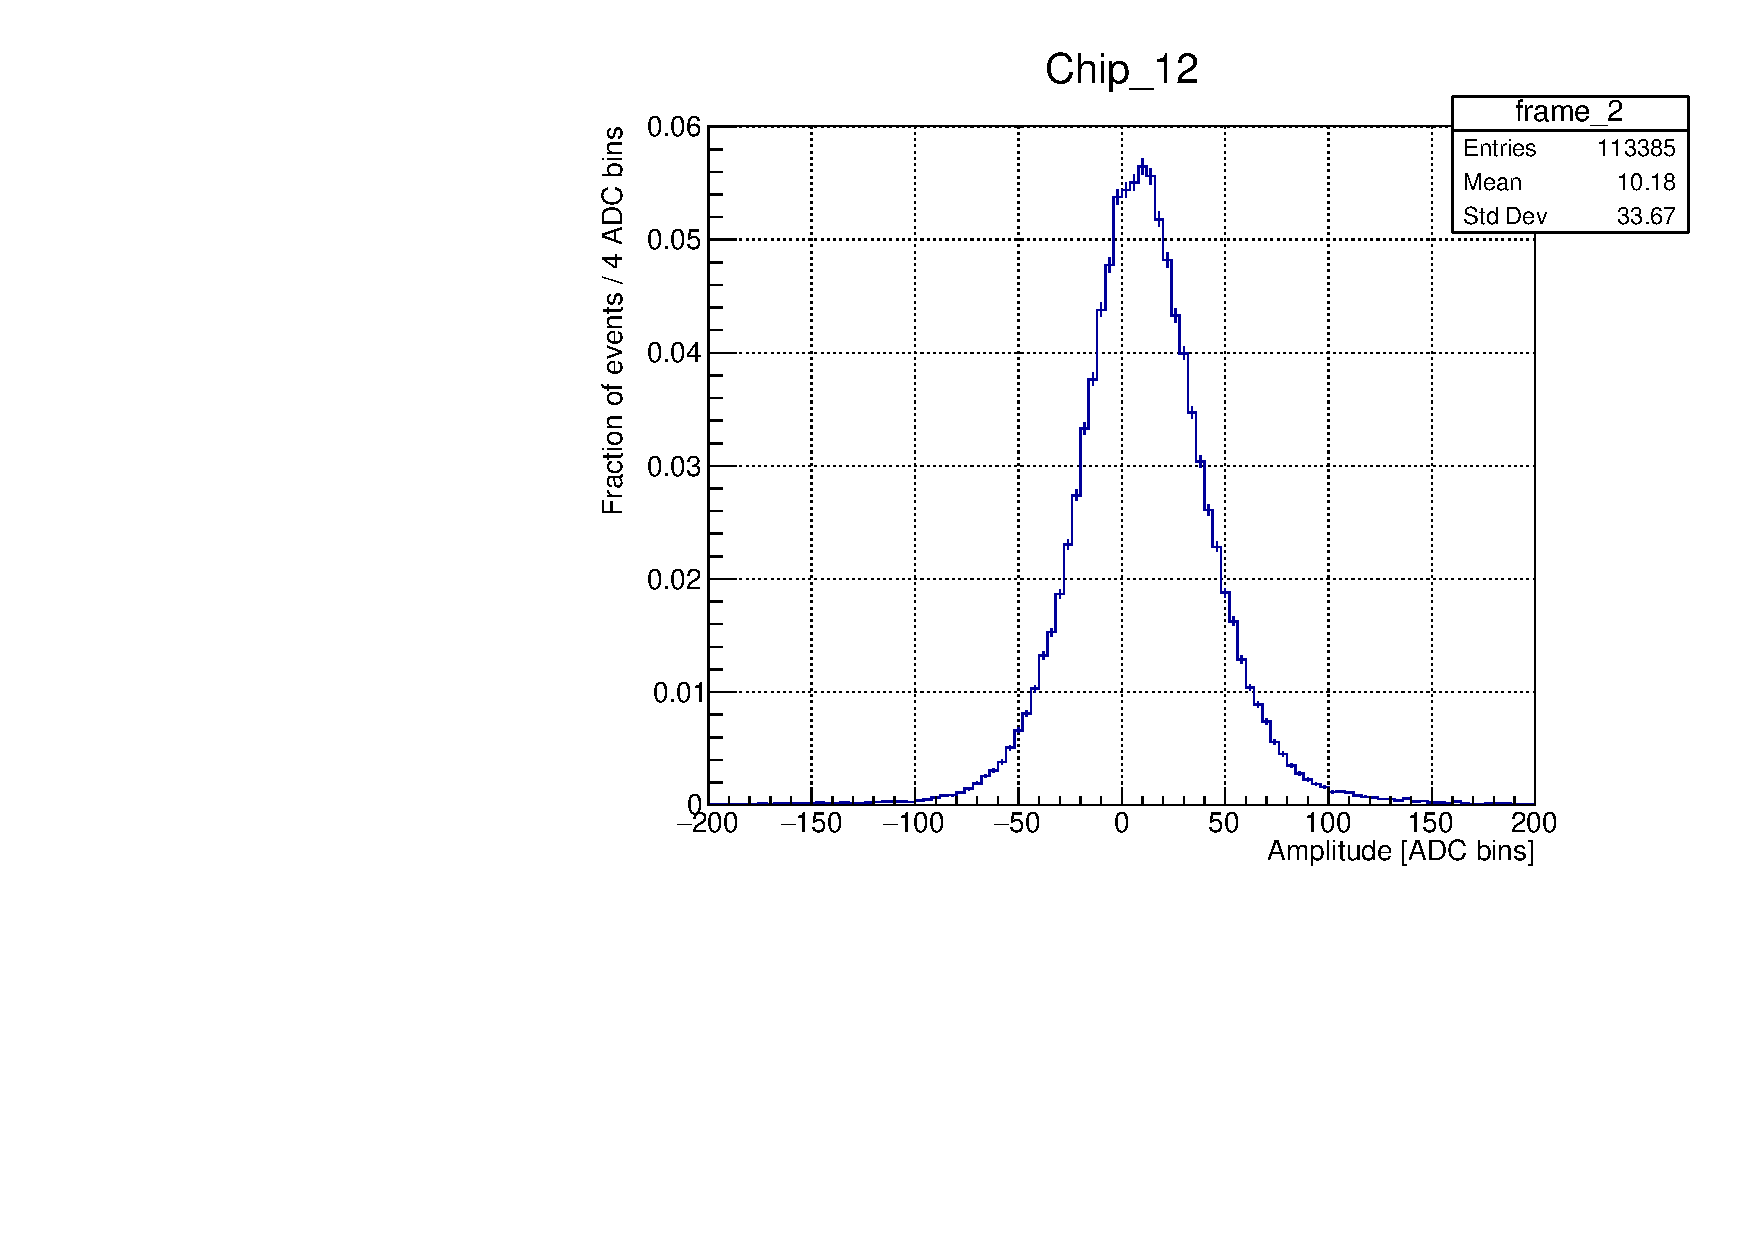
\includegraphics[width=\textwidth]{Chip_12_amp_hist}
	\end{subfigure}
	\caption{Амплитудные распределения событий различных чипов. Для анализа взят второй кадр}
	\label{fig:h_noise}
\end{figure}

\begin{figure}[t]
	\centering
	\begin{subfigure}[t]{0.45\textwidth}
		\centering
		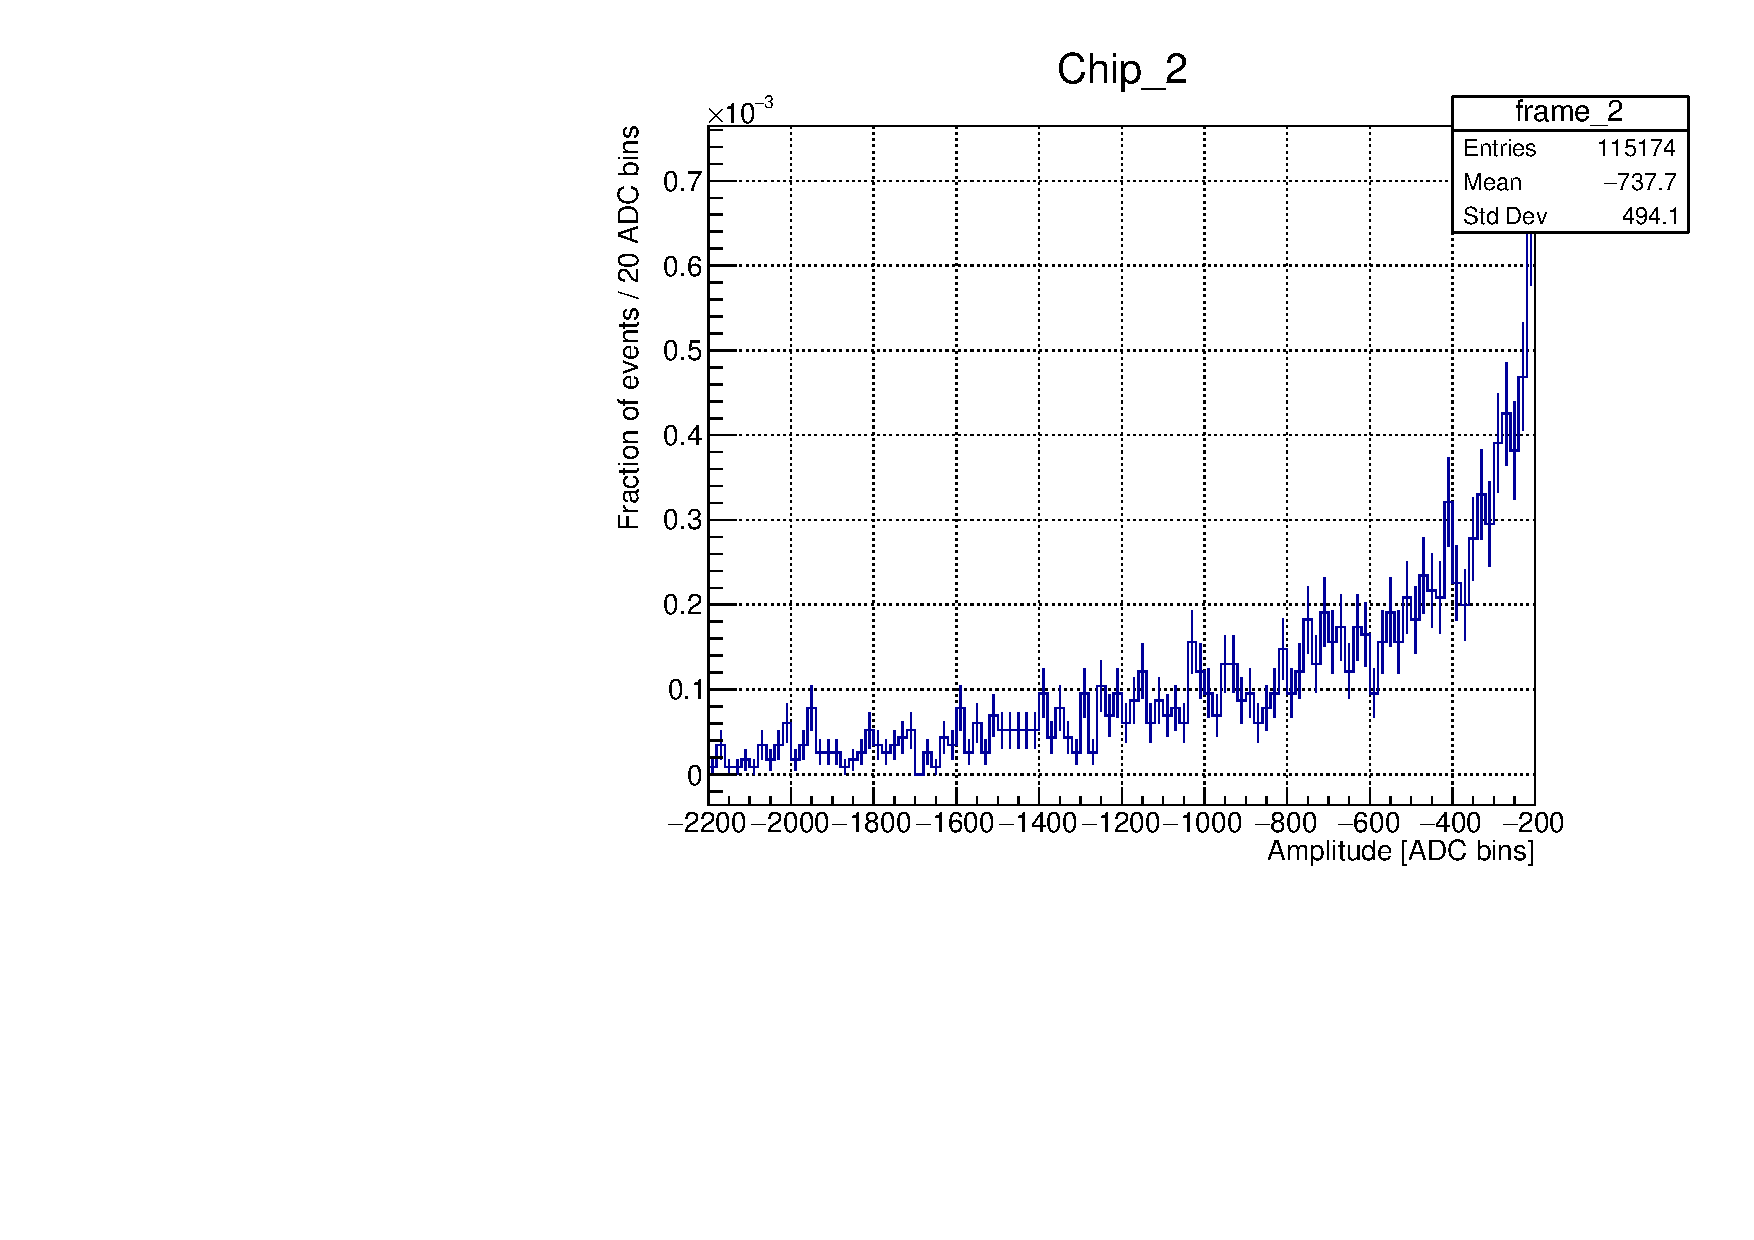
\includegraphics[width=\textwidth]{Chip_2_amp_hist_eff}
	\end{subfigure}
	\begin{subfigure}[t]{0.45\textwidth}
		\centering
		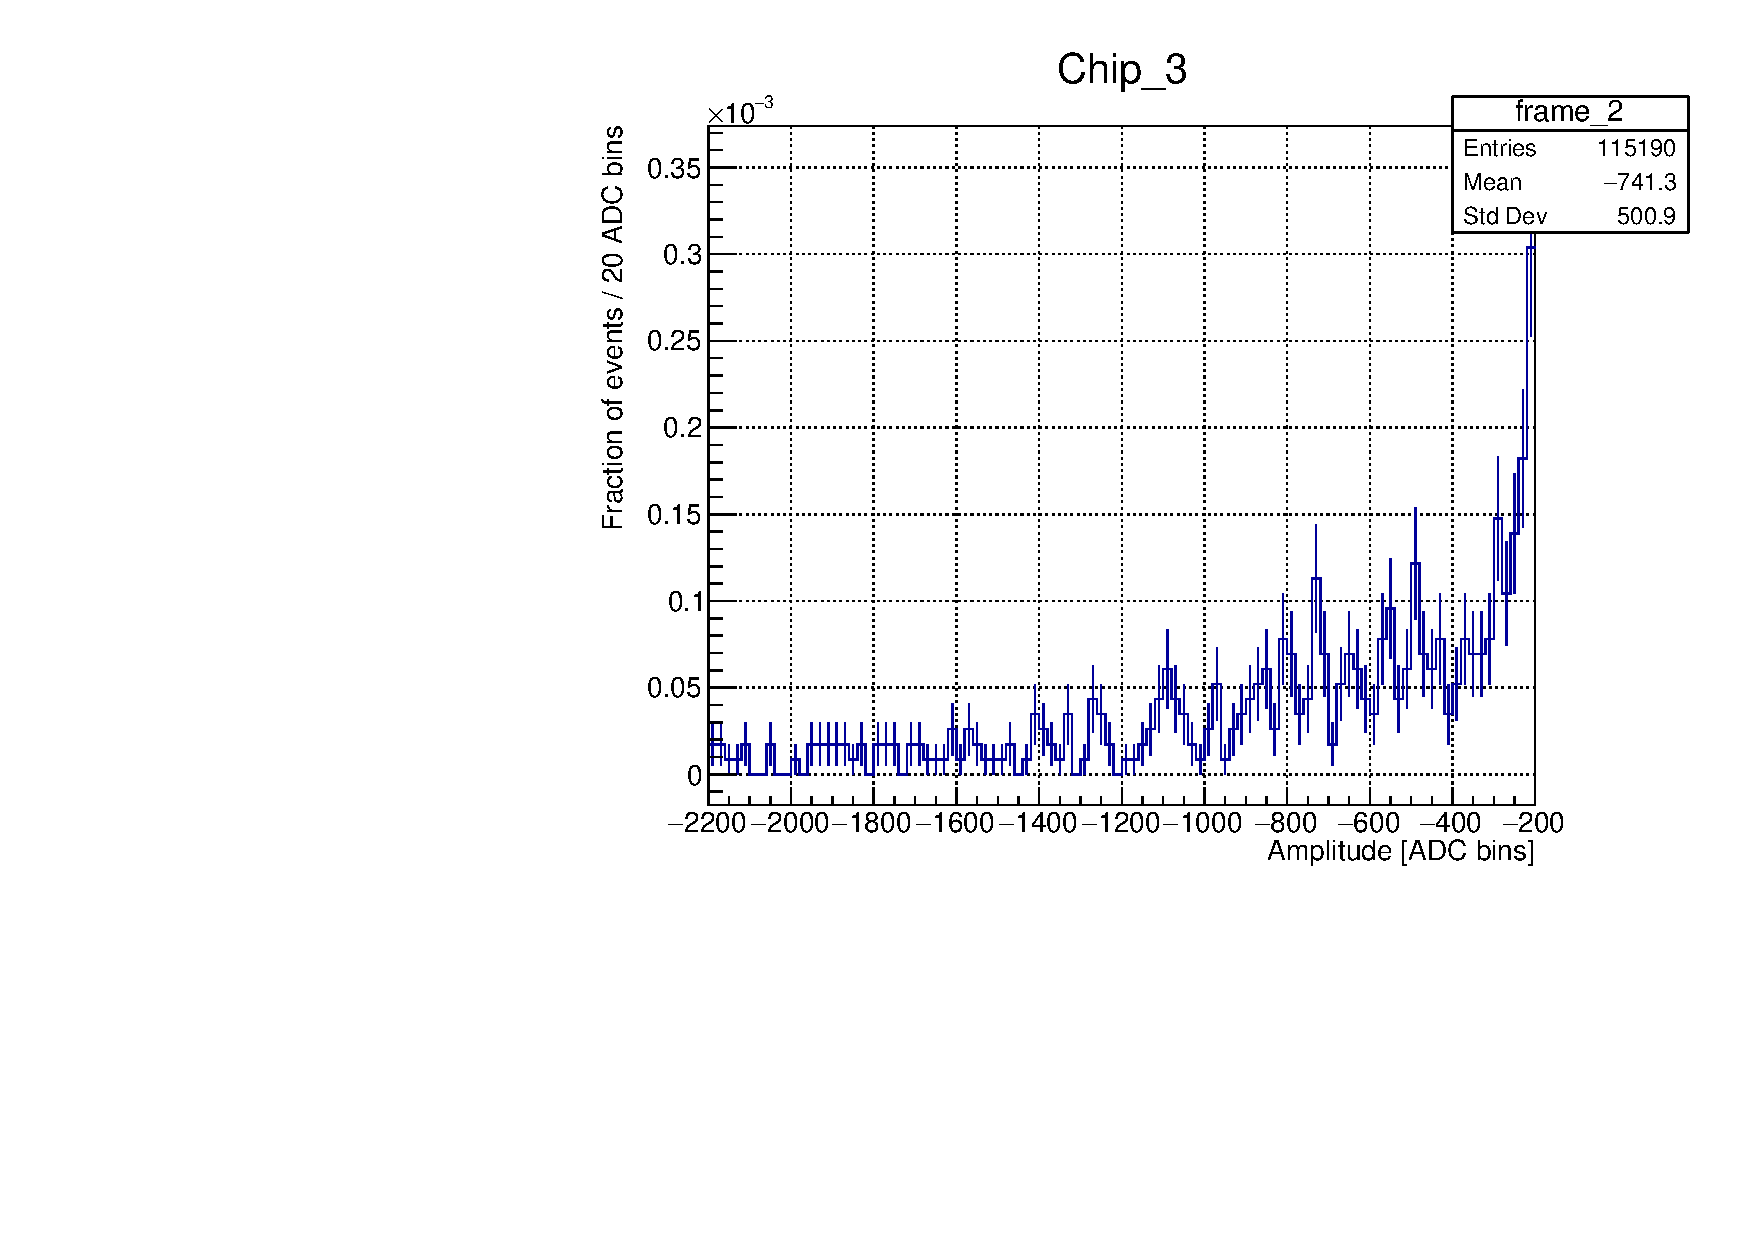
\includegraphics[width=\textwidth]{Chip_3_amp_hist_eff}
	\end{subfigure}
	\begin{subfigure}[t]{0.45\textwidth}
		\centering
		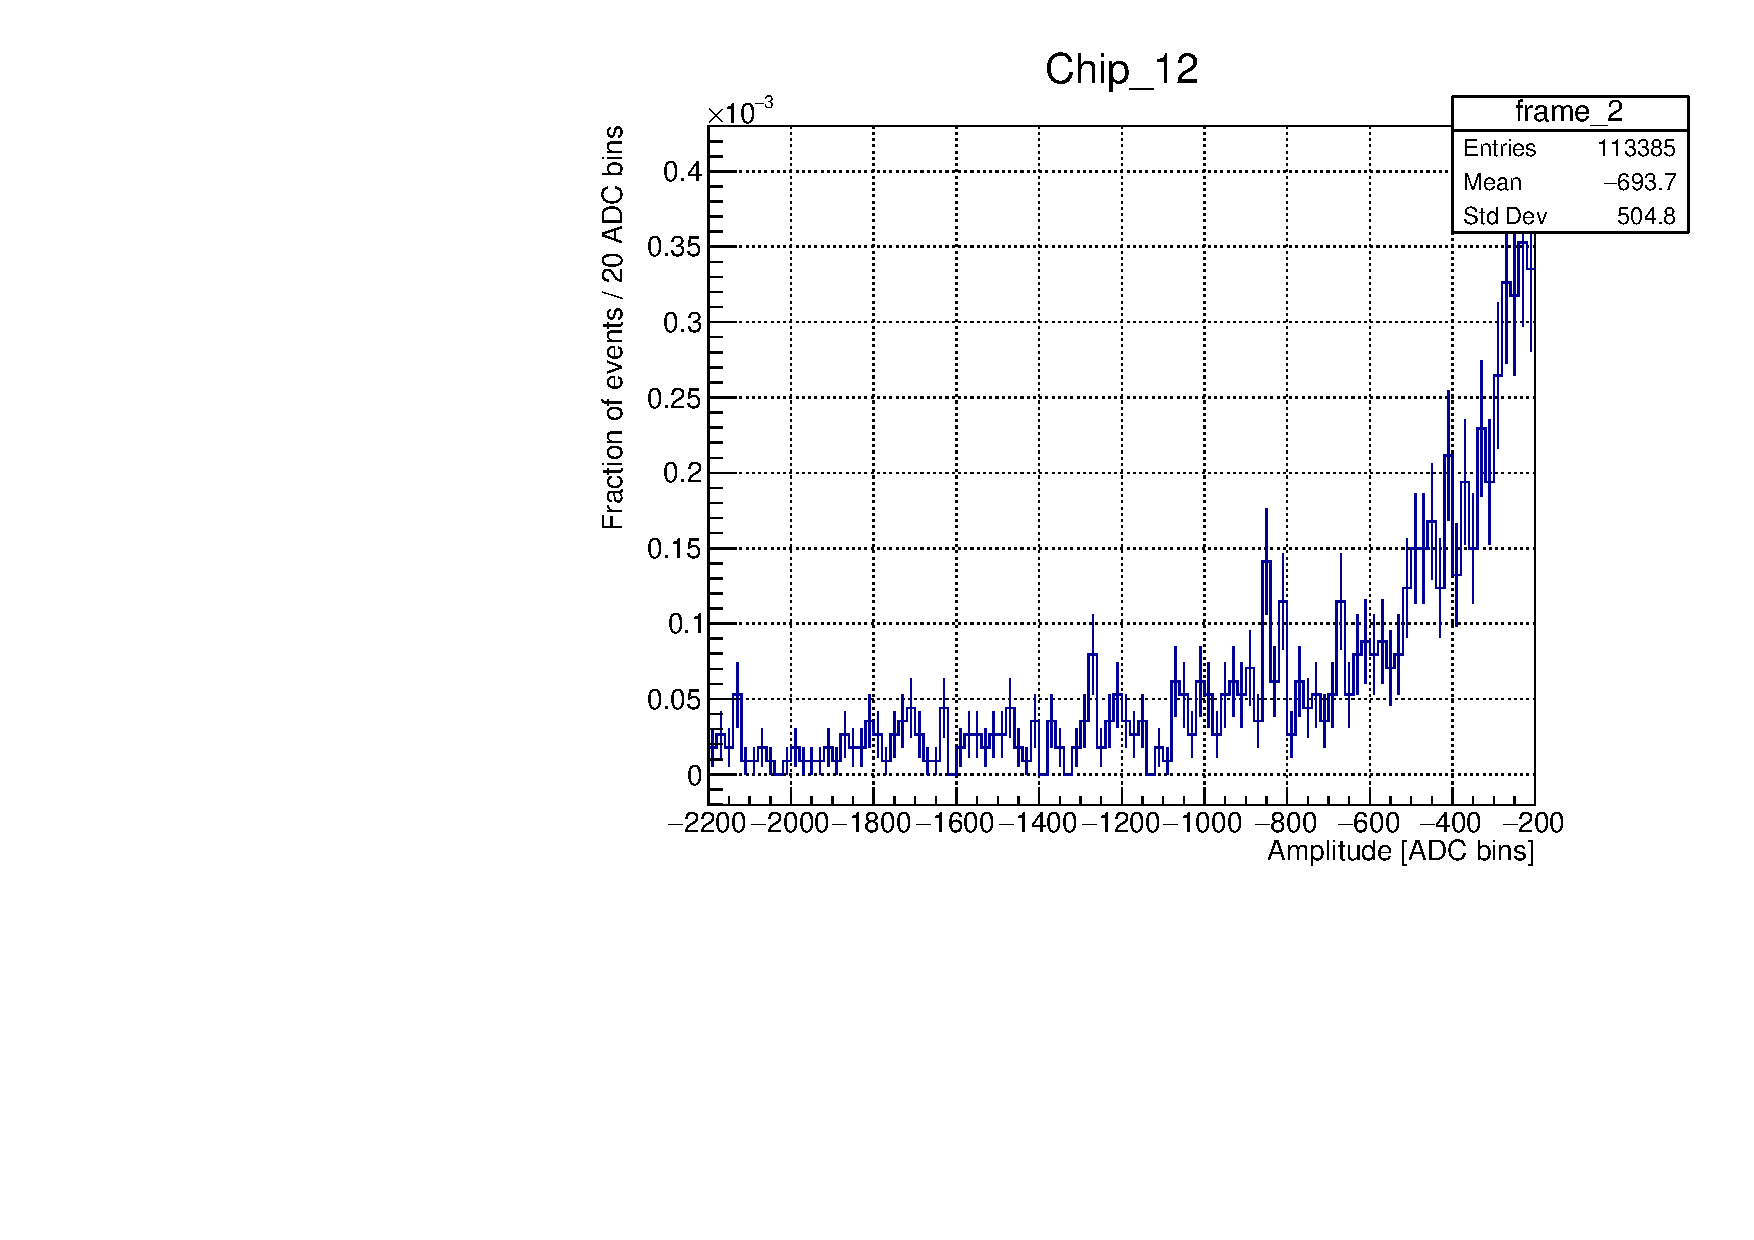
\includegraphics[width=\textwidth]{Chip_12_amp_hist_eff}
	\end{subfigure}
	\caption{Амплитудные распределения событий различных чипов. Область значений амплитуд не включает шумовой пик. Для анализа взят второй кадр.}
	\label{fig:h_sig}
\end{figure}

\vfill
\end{document}
